\documentclass[a4paper,14pt]{extarticle} %,twoside

%% Новые переменные, которые могут использоваться во всём проекте
\newcommand{\authorbibtitle}{Публикации автора по теме диссертации}
\newcommand{\fullbibtitle}{Список литературы} % (ГОСТ Р 7.0.11-2011, 4)

\newcommand{\ccbar}{\ensuremath{c\overline{c}}\xspace}
\newcommand{\nb}{\ensuremath{~\text{нб}}\xspace}
\newcommand{\pn}{\ensuremath{P^0}\xspace}
\newcommand{\dn}{\ensuremath{D^0}\xspace}
\newcommand{\bn}{\ensuremath{B^0}\xspace}
\newcommand{\hn}{\ensuremath{h^0}\xspace}
\newcommand{\dbar}{\ensuremath{\overline{D}}\xspace}
\newcommand{\pbar}{\ensuremath{\overline{P}}\xspace}
\newcommand{\bbar}{\ensuremath{\overline{B}}\xspace}
\newcommand{\fbar}{\ensuremath{\overline{f}}\xspace}
\newcommand{\qbar}{\ensuremath{\overline{q}}\xspace}
\newcommand{\bbbar}{\ensuremath{B\bbar}\xspace}
\newcommand{\qqbar}{\ensuremath{q\qbar}\xspace}
\newcommand{\ddbar}{\ensuremath{D\dbar}\xspace}
\newcommand{\dnbar}{\ensuremath{\dbar{}^0}\xspace}
\newcommand{\bnbar}{\ensuremath{\bbar{}^0}\xspace}
\newcommand{\pnbar}{\ensuremath{\pbar{}^0}\xspace}
\newcommand{\dstn}{\ensuremath{D^{*0}}\xspace}
\newcommand{\dstp}{\ensuremath{D^{*+}}\xspace}
\newcommand{\dstm}{\ensuremath{D^{*-}}\xspace}
\newcommand{\dstarn}{\ensuremath{D^{(*)0}}\xspace}
\newcommand{\dstnbar}{\ensuremath{\dbar{}^{*0}}\xspace}
\newcommand{\dstarnbar}{\ensuremath{\dbar{}^{(*)0}}\xspace}
\newcommand{\ks}{\ensuremath{K_S^0}\xspace}
\newcommand{\pip}{\ensuremath{\pi^+}\xspace}
\newcommand{\pim}{\ensuremath{\pi^-}\xspace}
\newcommand{\pin}{\ensuremath{\pi^0}\xspace}
\newcommand{\kstopipi}{\ensuremath{\ks\to\pip\pim}\xspace}
\newcommand{\cms}{\ensuremath{\textrm{СЦМ}}\xspace}


\newcommand{\prm}{\ensuremath{{}^{\prime}}\xspace}
\newcommand{\pprm}{\ensuremath{{}^{\prime\prime}}\xspace}
\newcommand{\ppprm}{\ensuremath{{}^{\prime\prime\prime}}\xspace}

\newcommand{\aphi}{\ensuremath{\alpha}\xspace}
\newcommand{\pphi}{\ensuremath{\beta}\xspace}
\newcommand{\gphi}{\ensuremath{\gamma}\xspace}
\newcommand{\sindbeta}{\ensuremath{\sin{2\pphi}}\xspace}
\newcommand{\cosdbeta}{\ensuremath{\cos{2\pphi}}\xspace}
%\newcommand{\pphib}{\ensuremath{\varphi_2}\xspace}
%\newcommand{\pphig}{\ensuremath{\varphi_3}\xspace}
\newcommand{\pphieff}{\ensuremath{\pphi_{\mathrm{eff}}}\xspace}
\newcommand{\sindbetaeff}{\ensuremath{\sin{2\pphieff}}\xspace}

\newcommand{\gamb}{\ensuremath{\Gamma_B}\xspace}
\newcommand{\gamt}{\ensuremath{\Gamma t}\xspace}
\newcommand{\gamdt}{\ensuremath{\Gamma_Dt}\xspace}
\newcommand{\gambt}{\ensuremath{\gamb t}\xspace}
\newcommand{\oxdydtsq}{\ensuremath{\mco\left((\gamdt)^2(x_D+y_D)^2\right)}\xspace}
\newcommand{\oxdydsq}{\ensuremath{\mco\left(x_D+y_D\right)^2}\xspace}
\newcommand{\orbxdyd}{\ensuremath{\mco\lbr\rb\lbr x_D+y_D\rbr\rbr}\xspace}
\newcommand{\emdgd}{\ensuremath{e^{-im_Dt-\frac{\gamdt}{2}}}\xspace}
\newcommand{\embgb}{\ensuremath{e^{-im_Bt-\frac{\gambt}{2}}}\xspace}
\newcommand{\emg}{\ensuremath{e^{-imt-\frac{\gamt}{2}}}\xspace}

\newcommand{\lbr}{\ensuremath{\left(}}
\newcommand{\rbr}{\ensuremath{\right)}}

\newcommand{\rcp}{\ensuremath{r_{\cpconj}}}
\newcommand{\alcp}{\ensuremath{\alpha_{\cpconj}}}
    
\newcommand{\bdk}{\ensuremath{B^{\pm}\to D K^{\pm}}\xspace}
\newcommand{\bdkp}{\ensuremath{B^+\to D K^+}\xspace}
\newcommand{\bdnkp}{\ensuremath{B^+\to\dn K^+}\xspace}
\newcommand{\bdbkp}{\ensuremath{B^+\to\dnbar K^+}\xspace}
\newcommand{\bdnkm}{\ensuremath{B^-\to\dn K^-}\xspace}
\newcommand{\bdbkm}{\ensuremath{B^-\to\dnbar K^-}\xspace}
\newcommand{\bdkm}{\ensuremath{B^-\to D K^-}\xspace}
\newcommand{\bdcpk}{\ensuremath{B^+\to D_{\cpconj} K^+}\xspace}

\newcommand{\delf}{\ensuremath{\Delta\delta_f}\xspace}
\newcommand{\deld}{\ensuremath{\Delta\delta_D}\xspace}
\newcommand{\delb}{\ensuremath{\Delta\delta_B}\xspace}
\newcommand{\rb}{\ensuremath{r_B}\xspace}
\newcommand{\rd}{\ensuremath{r_D}\xspace}
\newcommand{\mbc}{\ensuremath{M_{\mathrm{bc}}}\xspace}
\newcommand{\de}{\ensuremath{\Delta E}\xspace}
\newcommand{\dm}{\ensuremath{\Delta m}\xspace}
\newcommand{\dg}{\ensuremath{\Delta\Gamma}\xspace}
\newcommand{\debk}{\ensuremath{\left(\Delta E\right)}\xspace}

\newcommand{\br}{\ensuremath{\mathcal{B}}\xspace}
\newcommand{\dkpi}{\ensuremath{D\to K^+\pi^-}\xspace}
\newcommand{\dkpbar}{\ensuremath{D\to K^-\pi^+}\xspace}

\newcommand{\dd}{\ensuremath{\mathrm{d}}\xspace}
\newcommand{\ddlz}{\dd\mpsq\dd\mmsq}

\newcommand{\vckm}{\ensuremath{V_{\mathrm{CKM}}}\xspace}
\newcommand{\cabang}{\ensuremath{\theta_{\mathrm{C}}}\xspace}

\newcommand{\kspp}{\ensuremath{\ks\pi^+\pi^-}\xspace}
\newcommand{\kppn}{\ensuremath{K^-\pi^+\pin}\xspace}
\newcommand{\dkpp}{\ensuremath{D\to\ks\pi^+\pi^-}\xspace}
\newcommand{\dnkpp}{\ensuremath{\dn\to\ks\pi^+\pi^-}\xspace}
\newcommand{\dbkpp}{\ensuremath{\dnbar\to\ks\pi^+\pi^-}\xspace}
\newcommand{\dkspp}{\ensuremath{\dn\to\ks\pi^+\pi^-}\xspace}

\newcommand{\bpdrho}{\ensuremath{B^+\to\dnbar\rho^+}\xspace}
\newcommand{\bpdstarrho}{\ensuremath{B^+\to\dstarnbar\rho^+}\xspace}
\newcommand{\bpdstarpi}{\ensuremath{B^+\to\dstarnbar\pi^+}\xspace}
\newcommand{\bpdstph}{\ensuremath{B^+\to\dstp\hn}\xspace}

\newcommand{\bmdrho}{\ensuremath{B^-\to\dn\rho^-}\xspace}
\newcommand{\bmdstpi}{\ensuremath{B^-\to\dstm\pin}\xspace}
\newcommand{\bmdstrho}{\ensuremath{B^-\to\dstn\rho^-}\xspace}
\newcommand{\bmdstarrho}{\ensuremath{B^-\to\dstarn\rho^-}\xspace}
\newcommand{\bmdstph}{\ensuremath{B^-\to\dstm\hn}\xspace}

\newcommand{\etap}{\ensuremath{\eta^{\prime}}\xspace}

\newcommand{\bbdsth}{\ensuremath{\bnbar\to\dstarn\hn}\xspace}
\newcommand{\bdh}{\ensuremath{\bn\to\dnbar\hn}\xspace}
\newcommand{\bdnh}{\ensuremath{\bn\to\dn\hn}\xspace}
\newcommand{\bdsth}{\ensuremath{\bn\to\dstarnbar\hn}\xspace}
\newcommand{\bdstarh}{\ensuremath{\bn\to\dstnbar\hn}\xspace}
\newcommand{\bdpi}{\ensuremath{\bn\to\dnbar\pin}\xspace}
\newcommand{\bdeta}{\ensuremath{\bn\to\dnbar\eta}\xspace}
%\newcommand{\bdetagg}{\ensuremath{\bn\to\dnbar\eta_{\gamma\gamma}}\xspace}
\newcommand{\bdetagg}{\ensuremath{\bn\to\dnbar[\gamma\gamma]_{\eta}}\xspace}
\newcommand{\bdstaretagg}{\ensuremath{\bn\to\dstarnbar[\gamma\gamma]_{\eta}}\xspace}
\newcommand{\bdetap}{\ensuremath{\bn\to\dnbar\etap}\xspace}
\newcommand{\bdetappp}{\ensuremath{\bn\to\dnbar[\pi^+\pi^-\pi^0]_{\eta}}\xspace}
\newcommand{\bdomega}{\ensuremath{\bn\to\dnbar\omega}\xspace}
\newcommand{\bdstpi}{\ensuremath{\bn\to\dstnbar\pin}\xspace}
\newcommand{\bdstarpi}{\ensuremath{\bn\to\dstarnbar\pin}\xspace}
\newcommand{\bdsteta}{\ensuremath{\bn\to\dstnbar\eta}\xspace}

\newcommand{\bdpp}{\ensuremath{\bn\to D\pi^+\pi^-}\xspace}
\newcommand{\bdbpp}{\ensuremath{\bn\to \dnbar\pi^+\pi^-}\xspace}
\newcommand{\bbdpp}{\ensuremath{\bnbar\to \dn\pi^+\pi^-}\xspace}

\newcommand{\bpdpi}{\ensuremath{B^{+}\to\dnbar\pi^+}\xspace}
\newcommand{\bpdk}{\ensuremath{B^{+}\to\dnbar K^+}\xspace}

\newcommand{\dpp}{\ensuremath{\dn\pi^+\pi^-}\xspace}
\newcommand{\dbpp}{\ensuremath{\dnbar\pi^+\pi^-}\xspace}
\newcommand{\abdbpp}{\ensuremath{\mca_{\dbpp}}\xspace}
\newcommand{\abbdpp}{\ensuremath{\overline{\mca}{}_{\dpp}}\xspace}

\newcommand{\ppsi}{\ensuremath{\psi\lbr3770\rbr}\xspace}
\newcommand{\pppsi}{\ensuremath{\psi\lbr4040\rbr}\xspace}

\newcommand{\dpi}{\ensuremath{\dn\pin}\xspace}
\newcommand{\dstpi}{\ensuremath{\dstn\pin}\xspace}
\newcommand{\dsteta}{\ensuremath{\dstn\eta}\xspace}
\newcommand{\detagg}{\ensuremath{\dn\etasubgg}\xspace}
\newcommand{\detap}{\ensuremath{\dn\etap}\xspace}
\newcommand{\detappp}{\ensuremath{\dn\etasubppp}\xspace}
\newcommand{\domega}{\ensuremath{\dn\omega}\xspace}
\newcommand{\todstpi}{\ensuremath{\dstn\pin}\xspace}
\newcommand{\todsteta}{\ensuremath{\dstn\eta}\xspace}
\newcommand{\etapetapp}{\ensuremath{\etap\to[\gamma\gamma]_{\eta}\pi^+\pi^-}\xspace}
\newcommand{\dstdpi}{\ensuremath{\dstn\to\dn\pin}\xspace}
\newcommand{\dbstdbpi}{\ensuremath{\dbar{}^{*0}\to\dnbar\pin}\xspace}

\newcommand{\dstpdpip}{\ensuremath{\dstp\to\dn\pi^+}\xspace}

\newcommand{\jpsi}{\ensuremath{J/\psi}\xspace}
\newcommand{\psiss}{\ensuremath{\psi(2S)}\xspace}
\newcommand{\bjpsiks}{\ensuremath{\bn\to\jpsi\ks}\xspace}
\newcommand{\bjpsikstar}{\ensuremath{\bn\to\jpsi K^*}\xspace}
\newcommand{\bpsissks}{\ensuremath{\bn\to\psiss\ks}\xspace}
\newcommand{\bddks}{\ensuremath{\bn\to D^{(*)}D^{(*)}\ks}\xspace}
\newcommand{\bsjpsiphi}{\ensuremath{B_s\to \jpsi\varphi}\xspace}

\newcommand{\vud}{\ensuremath{V_{ub}}\xspace}
\newcommand{\vus}{\ensuremath{V_{us}}\xspace}
\newcommand{\vub}{\ensuremath{V_{ub}}\xspace}

\newcommand{\vcd}{\ensuremath{V_{cd}}\xspace}
\newcommand{\vcs}{\ensuremath{V_{cs}}\xspace}
\newcommand{\vcb}{\ensuremath{V_{cb}}\xspace}

\newcommand{\vtd}{\ensuremath{V_{td}}\xspace}
\newcommand{\vts}{\ensuremath{V_{ts}}\xspace}
\newcommand{\vtb}{\ensuremath{V_{tb}}\xspace}

\newcommand{\vudst}{\ensuremath{V_{ud}^*}\xspace}
\newcommand{\vusst}{\ensuremath{V_{us}^*}\xspace}
\newcommand{\vubst}{\ensuremath{V_{ub}^*}\xspace}

\newcommand{\vcdst}{\ensuremath{V_{cd}^*}\xspace}
\newcommand{\vcsst}{\ensuremath{V_{cs}^*}\xspace}
\newcommand{\vcbst}{\ensuremath{V_{cb}^*}\xspace}

\newcommand{\dedx}{\ensuremath{\mathrm{d}E/\mathrm{d}x}\xspace}

\newcommand{\vtdst}{\ensuremath{V_{td}^*}\xspace}
\newcommand{\vtsst}{\ensuremath{V_{ts}^*}\xspace}
\newcommand{\vtbst}{\ensuremath{V_{tb}^*}\xspace}

\newcommand{\mosq}{\ensuremath{m_{12}^2}\xspace}
\newcommand{\mtsq}{\ensuremath{m_{13}^2}\xspace}
\newcommand{\mpsq}{\ensuremath{m_+^2}\xspace}
\newcommand{\mmsq}{\ensuremath{m_-^2}\xspace}
\newcommand{\mpmsq}{\ensuremath{m_{\pm}^2}\xspace}
\newcommand{\mmpsq}{\ensuremath{m_{\mp}^2}\xspace}
\newcommand{\mupsq}{\ensuremath{\mu_+^2}\xspace}
\newcommand{\mumsq}{\ensuremath{\mu_-^2}\xspace}

\newcommand{\bg}{\ensuremath{\lbr \beta\gamma \rbr}\xspace}
\newcommand{\cbgups}{\ensuremath{c\bg_{\ups}}\xspace}
\newcommand{\bgups}{\ensuremath{\bg_{\ups}}\xspace}

\newcommand{\ak}{\ensuremath{a_{\mathrm{k}}}\xspace}
\newcommand{\ck}{\ensuremath{c_{\mathrm{k}}}\xspace}

\newcommand{\albf}{\ensuremath{\boldsymbol{\alpha}}\xspace}
\newcommand{\vbf}{\ensuremath{\mathbf{v}}\xspace}
\newcommand{\Hbf}{\ensuremath{\mathbf{H}}\xspace}
\newcommand{\Vbf}{\ensuremath{\mathbf{V}}\xspace}

\newcommand{\detr}{\ensuremath{\mathrm{detr}}\xspace}
\newcommand{\np}{\ensuremath{\mathrm{np}}\xspace}
\newcommand{\kin}{\ensuremath{\mathrm{k}}\xspace}

\newcommand{\rmq}{\ensuremath{\mathrm{q}}\xspace}
\newcommand{\rmp}{\ensuremath{\mathrm{p}}\xspace}
\newcommand{\rmn}{\ensuremath{\mathrm{n}}\xspace}

\newcommand{\motsq}{\ensuremath{\lbr\mosq,\mtsq\rbr}\xspace}
\newcommand{\mottsq}{\ensuremath{\lbr\mosq,\mtsq,t\rbr}\xspace}

\newcommand{\dt}{\ensuremath{\Delta t}\xspace}
\newcommand{\dz}{\ensuremath{\Delta z}\xspace}
\newcommand{\dtp}{\ensuremath{\Delta t^{\prime}}\xspace}
\newcommand{\dtpp}{\ensuremath{\Delta t^{\prime\prime}}\xspace}
\newcommand{\dtppp}{\ensuremath{\Delta t^{\prime\prime\prime}}\xspace}
\newcommand{\dtj}{\ensuremath{\Delta t_{j}}\xspace}

\newcommand{\btoccq}{\ensuremath{b\to c\overline{c}q}\xspace}
\newcommand{\btoccd}{\ensuremath{b\to c\overline{c}d}\xspace}
\newcommand{\btoccs}{\ensuremath{b\to c\overline{c}s}\xspace}
\newcommand{\btoqqs}{\ensuremath{b\to q\overline{q}s}\xspace}
\newcommand{\btosss}{\ensuremath{b\to s\overline{s}s}\xspace}
\newcommand{\btossd}{\ensuremath{b\to s\overline{s}d}\xspace}
\newcommand{\btodds}{\ensuremath{b\to d\overline{d}s}\xspace}
\newcommand{\btoddd}{\ensuremath{b\to d\overline{d}d}\xspace}
\newcommand{\btocud}{\ensuremath{b\to c\overline{u}d}\xspace}
\newcommand{\btoucd}{\ensuremath{b\to u\overline{c}d}\xspace}
\newcommand{\btouud}{\ensuremath{b\to u\overline{u}d}\xspace}
\newcommand{\btouus}{\ensuremath{b\to u\overline{u}s}\xspace}
\newcommand{\btouuq}{\ensuremath{b\to u\overline{u}q}\xspace}
\newcommand{\btocus}{\ensuremath{b\to c\overline{u}s}\xspace}
\newcommand{\btoucs}{\ensuremath{b\to u\overline{c}s}\xspace}

\newcommand{\stat}{\ensuremath{\left({\textrm{стат}.}\right)}\xspace}
\newcommand{\syst}{\ensuremath{\left({\textrm{сист}.}\right)}\xspace}

\newcommand{\substat}{\ensuremath{{}_{\mathrm{stat}}}\xspace}
\newcommand{\subsyst}{\ensuremath{{}_{\mathrm{syst}}}\xspace}

\newcommand{\ep}{\ensuremath{e^+e^-}\xspace}
\newcommand{\vecp}{\ensuremath{\mathbf{p}}\xspace}

\newcommand{\cbfcn}{\ensuremath{G_{\mathrm{CB}}}\xspace}
\newcommand{\nskfcn}{\ensuremath{G_{\mathrm{Nsk}}}\xspace}
\newcommand{\erf}{\ensuremath{G_{\mathrm{erf}}}\xspace}

\newcommand{\thhel}{\ensuremath{\theta_{\mathrm{hel}}}\xspace}
\newcommand{\ththr}{\ensuremath{\theta_{\mathrm{thr}}}\xspace}

\newcommand{\mco}{\ensuremath{\mathcal{O}}\xspace}
\newcommand{\mcr}{\ensuremath{\mathcal{R}}\xspace}
\newcommand{\mcd}{\ensuremath{\mathcal{D}}\xspace}
\newcommand{\mcl}{\ensuremath{\mathcal{L}}\xspace}
\newcommand{\mck}{\ensuremath{\mathcal{K}}\xspace}
\newcommand{\mca}{\ensuremath{\mathcal{A}}\xspace}
\newcommand{\mcb}{\ensuremath{\mathcal{B}}\xspace}
\newcommand{\mcn}{\ensuremath{\mathcal{N}}\xspace}
\newcommand{\mcp}{\ensuremath{\mathcal{P}}\xspace}
\newcommand{\mcs}{\ensuremath{\mathcal{S}}\xspace}
\newcommand{\mcabar}{\ensuremath{\overline{\mca}}\xspace}
\newcommand{\mcpbar}{\ensuremath{\overline{\mcp}}\xspace}
\newcommand{\acp}{\ensuremath{\mca_\cpconj}\xspace}
\newcommand{\mcm}{\ensuremath{\mathcal{M}}\xspace}
\newcommand{\mcmbar}{\ensuremath{\overline{\mcm}}\xspace}

\newcommand{\mcpd}{\ensuremath{\mcp_D}\xspace}
\newcommand{\mcpdbar}{\ensuremath{\mcpbar_D}\xspace}

\newcommand{\ndf}{\ensuremath{\mathrm{n.d.f.}}\xspace}

\newcommand{\ad}{\ensuremath{\mca_D}}
\newcommand{\adbar}{\ensuremath{\mcabar_D}}
\newcommand{\dvar}{\ensuremath{\left(\mpsq,\mmsq\right)}\xspace}
\newcommand{\dvarinv}{\ensuremath{\left(\mmsq,\mpsq\right)}\xspace}
\newcommand{\advar}{\ensuremath{\ad\dvar}\xspace}
\newcommand{\advarinv}{\ensuremath{\ad\dvarinv}\xspace}
\newcommand{\advarinvconj}{\ensuremath{\mca^{*}_D\dvarinv}\xspace}
\newcommand{\adsq}{\ensuremath{\left|\ad\right|^2}\xspace}
\newcommand{\advarsq}{\ensuremath{\left|\ad\dvar)\right|^2}\xspace}
\newcommand{\advarinvsq}{\ensuremath{\left|\ad\dvarinv\right|^2}\xspace}

\newcommand{\pd}{\ensuremath{\mcp_D}}
\newcommand{\pdbar}{\ensuremath{\mcpbar_D}}

\newcommand{\ads}{\textrm{ADS}}
\newcommand{\glw}{\textrm{GLW}}

\newcommand{\imag}{\ensuremath{\mathrm{Im}}}

\newcommand{\ab}{\ensuremath{\mca_B}}
\newcommand{\abbar}{\ensuremath{\mcabar_B}}
\newcommand{\af}{\ensuremath{\mca_f}\xspace}
\newcommand{\afbar}{\ensuremath{\mcabar{}_f}\xspace}
\newcommand{\bvar}{\ensuremath{\left(\mupsq,\mumsq\right)}\xspace}
\newcommand{\bvarinv}{\ensuremath{\left(\mumsq,\mupsq\right)}\xspace}

\newcommand{\ddlzarea}{\ensuremath{\limits_{\mcd_i}}\xspace}

\newcommand{\cpconj}{\ensuremath{\mathcal{CP}}\xspace}
\newcommand{\pconj}{\ensuremath{\mathcal{P}}\xspace}
\newcommand{\cconj}{\ensuremath{\mathcal{C}}\xspace}
\newcommand{\tconj}{\ensuremath{\mathcal{T}}\xspace}
\newcommand{\cpvconj}{\ensuremath{\mathcal{CPV}}\xspace}
\newcommand{\cptconj}{\ensuremath{\mathcal{CPT}}\xspace}

\newcommand{\bz}{\ensuremath{\left|\bn\right>}\xspace}
\newcommand{\bzb}{\ensuremath{\left|\bnbar\right>}\xspace}
\newcommand{\ba}{\ensuremath{\left|B_H\right>}\xspace}
\newcommand{\bb}{\ensuremath{\left|B_L\right>}\xspace}

\newcommand{\rmh}{\ensuremath{\mathrm{H}}\xspace}
\newcommand{\rml}{\ensuremath{\mathrm{L}}\xspace}

\newcommand{\pz}{\ensuremath{\left|\pn\right>}\xspace}
\newcommand{\pzb}{\ensuremath{\left|\pnbar\right>}\xspace}
\newcommand{\pa}{\ensuremath{\left|P_{\rmh}\right>}\xspace}
\newcommand{\pb}{\ensuremath{\left|P_{\rml}\right>}\xspace}

\newcommand{\bzt}{\ensuremath{\left|\bn\left(t\right)\right>}\xspace}
\newcommand{\bzbt}{\ensuremath{\left|\bnbar\left(t\right)\right>}\xspace}
\newcommand{\bzta}{\ensuremath{\left|\bn\left(t_1\right)\right>}\xspace}
\newcommand{\bztb}{\ensuremath{\left|\bn\left(t_2\right)\right>}\xspace}
\newcommand{\bzbta}{\ensuremath{\left|\bnbar\left(t_1\right)\right>}\xspace}
\newcommand{\bzbtb}{\ensuremath{\left|\bnbar\left(t_2\right)\right>}\xspace}
\newcommand{\bat}{\ensuremath{\left|B_{\rmh}\left(t\right)\right>}\xspace}
\newcommand{\bbt}{\ensuremath{\left|B_{\rml}\left(t\right)\right>}\xspace}

\newcommand{\pzt}{\ensuremath{\left|\pn\left(t\right)\right>}\xspace}
\newcommand{\pzbt}{\ensuremath{\left|\pnbar\left(t\right)\right>}\xspace}
\newcommand{\pzta}{\ensuremath{\left|\pn\left(t_1\right)\right>}\xspace}
\newcommand{\pztb}{\ensuremath{\left|\pn\left(t_2\right)\right>}\xspace}
\newcommand{\pzbta}{\ensuremath{\left|\pnbar\left(t_1\right)\right>}\xspace}
\newcommand{\pzbtb}{\ensuremath{\left|\pnbar\left(t_2\right)\right>}\xspace}
\newcommand{\pat}{\ensuremath{\left|P_{\rmh}\left(t\right)\right>}\xspace}
\newcommand{\pbt}{\ensuremath{\left|P_{\rml}\left(t\right)\right>}\xspace}

\newcommand{\bzti}{\ensuremath{\left|\bn\left(0\right)\right>}\xspace}
\newcommand{\bzbti}{\ensuremath{\left|\bnbar\left(0\right)\right>}\xspace}
\newcommand{\bati}{\ensuremath{\left|B_{\rmh}\left(0\right)\right>}\xspace}
\newcommand{\bbti}{\ensuremath{\left|B_{\rml}\left(0\right)\right>}\xspace}

\newcommand{\pzti}{\ensuremath{\left|\pn\left(0\right)\right>}\xspace}
\newcommand{\pzbti}{\ensuremath{\left|\pnbar\left(0\right)\right>}\xspace}
\newcommand{\pati}{\ensuremath{\left|P_{\rmh}\left(0\right)\right>}\xspace}
\newcommand{\pbti}{\ensuremath{\left|P_{\rml}\left(0\right)\right>}\xspace}

\newcommand{\kapp}{\ensuremath{\varkappa\left(t\right)}\xspace}
\newcommand{\sigm}{\ensuremath{\sigma\left(t\right)}\xspace}

\newcommand{\kappb}{\ensuremath{\varkappa_B\left(t\right)}\xspace}
\newcommand{\sigmb}{\ensuremath{\sigma_B\left(t\right)}\xspace}

\newcommand{\kappd}{\ensuremath{\varkappa_D\left(t\right)}\xspace}
\newcommand{\sigmd}{\ensuremath{\sigma_D\left(t\right)}\xspace}

\newcommand{\rec}{\ensuremath{\mathrm{rec}}\xspace}
\newcommand{\asc}{\ensuremath{\mathrm{asc}}\xspace}

\newcommand{\bs}{\ensuremath{B_s^0}\xspace}

\newcommand{\ups}{\ensuremath{\Upsilon\left(4S\right)}\xspace}
\newcommand{\brec}{\ensuremath{B_{\rec}}\xspace}
\newcommand{\basc}{\ensuremath{B_{\asc}}\xspace}
\newcommand{\thrrec}{\ensuremath{\mathbf{T}_{\rec}}\xspace}
\newcommand{\thrasc}{\ensuremath{\mathbf{T}_{\asc}}\xspace}

\newcommand{\epseff}{\ensuremath{\varepsilon_{\mathrm{eff}}}\xspace}

\newcommand{\kapdt}{\ensuremath{\varkappa\left(\dt\right)}\xspace}
\newcommand{\sigdt}{\ensuremath{\sigma\left(\dt\right)}\xspace}

\newcommand{\hgg}{\ensuremath{\hn\to\gamma\gamma}\xspace}
\newcommand{\pigg}{\ensuremath{\pin\to\gamma\gamma}\xspace}
\newcommand{\dst}{\ensuremath{D^{*}(2007)^0}\xspace}
\newcommand{\etagg}{\ensuremath{\eta\to\gamma\gamma}\xspace}
\newcommand{\etasubgg}{\ensuremath{{[\gamma\gamma]}_{\eta}}\xspace}
\newcommand{\hppp}{\ensuremath{\hn\to\pi^+\pi^-\pi^0}\xspace}
\newcommand{\etappp}{\ensuremath{\eta\to\pi^+\pi^-\pi^0}\xspace}
\newcommand{\etasubppp}{\ensuremath{{[\pi^+\pi^-\pi^0]}_{\eta}}\xspace}
\newcommand{\omegappp}{\ensuremath{\omega\to\pi^+\pi^-\pi^0}\xspace}
\newcommand{\omegasubppp}{\ensuremath{\omega_{\pi^+\pi^-\pi^0}}\xspace}

\newcommand{\ifb}{\ensuremath{~\textrm{фбн}^{-1}}\xspace}
\newcommand{\mev}{\ensuremath{~\textrm{МэВ}}\xspace}
\newcommand{\gev}{\ensuremath{~\textrm{ГэВ}}\xspace}
\newcommand{\mevc}{\ensuremath{\mev/c}\xspace}
\newcommand{\gevc}{\ensuremath{\gev/c}\xspace}
\newcommand{\mevcsq}{\ensuremath{\mevc^{2}}\xspace}
\newcommand{\gevcsq}{\ensuremath{\gevc^{2}}\xspace}
\newcommand{\cm}{\ensuremath{~\textrm{см}}\xspace}
\newcommand{\mm}{\ensuremath{~\textrm{мм}}\xspace}
%\newcommand{\s}{\ensuremath{~\textrm{с}}\xspace}
\newcommand{\gz}{\ensuremath{~\textrm{Гц}}\xspace}
\newcommand{\lumi}{\ensuremath{~\textrm{см}^{-2}\textrm{с}^{-1}}\xspace}
\newcommand{\ps}{\ensuremath{~\textrm{пс}}\xspace}
\newcommand{\mum}{\ensuremath{~\textrm{мкм}}\xspace}
\newcommand{\mus}{\ensuremath{~\textrm{мкс}}\xspace}
\newcommand{\mdz}{\ensuremath{~\textrm{МДж}}\xspace}

\newcommand{\argus}{\ensuremath{p_{\mathrm{Argus}}}\xspace}
\newcommand{\cheb}{\ensuremath{T_2}\xspace}

\newcommand{\lab}{\ensuremath{\mathrm{lab}}\xspace}

\newcommand{\sig}{\ensuremath{\mathrm{sig}}\xspace}
\newcommand{\cnt}{\ensuremath{\mathrm{cnt}}\xspace}
\newcommand{\cmb}{\ensuremath{\mathrm{cmb}}\xspace}
\newcommand{\bkg}{\ensuremath{\mathrm{bkg}}\xspace}
\newcommand{\tot}{\ensuremath{\mathrm{tot}}\xspace}
\newcommand{\gen}{\ensuremath{\mathrm{gen}}\xspace}

\newcommand{\expr}{\ensuremath{\mathrm{exp}}\xspace}
\newcommand{\nuis}{\ensuremath{\mathrm{nuis}}\xspace}

\newcommand{\subsig}{\ensuremath{{}_{\sig}}\xspace}
\newcommand{\subcnt}{\ensuremath{{}_{\cnt}}\xspace}
\newcommand{\subcmb}{\ensuremath{{}_{\cmb}}\xspace}
\newcommand{\subbkg}{\ensuremath{{}_{\bkg}}\xspace}
\newcommand{\subtot}{\ensuremath{{}_{\tot}}\xspace}

\newcommand{\peak}{\ensuremath{\mathrm{peak}}\xspace}
\newcommand{\main}{\ensuremath{\mathrm{main}}\xspace}
\newcommand{\tail}{\ensuremath{\mathrm{tail}}\xspace}
\newcommand{\subpeak}{\ensuremath{{}_{\peak}}\xspace}
\newcommand{\subtail}{\ensuremath{{}_{\tail}}\xspace}

\newcommand{\psig}{\ensuremath{p\subsig}\xspace}
\newcommand{\isig}{\ensuremath{I\subsig}\xspace}
\newcommand{\nsig}{\ensuremath{N\subsig}\xspace}
\newcommand{\fsig}{\ensuremath{f\subsig}\xspace}
%\newcommand{\fsigj}{\ensuremath{f_{{\mathrm{sig}},j}}\xspace}
\newcommand{\fsigj}{\ensuremath{f^j_{\mathrm{sig}}}\xspace}

%\newcommand{\fqqj}{\ensuremath{f_{{\mathrm{qq}},j}}\xspace}
\newcommand{\fqqj}{\ensuremath{f^j_{\mathrm{qq}}}\xspace}

\newcommand{\pcnt}{\ensuremath{p\subcnt}\xspace}
\newcommand{\icnt}{\ensuremath{I\subcnt}\xspace}
\newcommand{\ncnt}{\ensuremath{N\subcnt}\xspace}
\newcommand{\fcnt}{\ensuremath{f\subcnt}\xspace}

\newcommand{\pcmb}{\ensuremath{p\subcmb}\xspace}
\newcommand{\icmb}{\ensuremath{I\subcmb}\xspace}
\newcommand{\ncmb}{\ensuremath{N\subcmb}\xspace}
\newcommand{\fcmb}{\ensuremath{f\subcmb}\xspace}

\newcommand{\ppeak}{\ensuremath{p\subpeak}\xspace}
\newcommand{\ipeak}{\ensuremath{I\subpeak}\xspace}
\newcommand{\npeak}{\ensuremath{N\subpeak}\xspace}
\newcommand{\fpeak}{\ensuremath{f\subpeak}\xspace}

\newcommand{\tbkg}{\ensuremath{\tau\subbkg}\xspace}

\newcommand{\ntot}{\ensuremath{N\subtot}\xspace}
\newcommand{\nbkg}{\ensuremath{N\subbkg}\xspace}
\newcommand{\pbkg}{\ensuremath{p\subbkg}\xspace}
\newcommand{\fbkg}{\ensuremath{f\subbkg}\xspace}
\newcommand{\fbkgj}{\ensuremath{f_{{\mathrm{bkg}},j}}\xspace}

\newcommand{\rphi}{\ensuremath{r\varphi}\xspace}
\newcommand{\pt}{\ensuremath{p_{\mathrm{T}}}\xspace}
\newcommand{\pl}{\ensuremath{p_{\mathrm{L}}}\xspace}

\newcommand{\csit}{\ensuremath{\mathrm{CsI}(\mathrm{Tl})}\xspace}
\newcommand{\sdsp}{\ensuremath{\textrm{МФОС}}\xspace}
\newcommand{\fpga}{\ensuremath{\textrm{ППВМ}}\xspace}

\newcommand{\svd}{\ensuremath{\textrm{ВД}}\xspace}
\newcommand{\dssd}{\ensuremath{\textrm{ДКПД}}\xspace}
\newcommand{\cdc}{\ensuremath{\textrm{ЦДК}}\xspace}
\newcommand{\acc}{\ensuremath{\textrm{АЧС}}\xspace}
\newcommand{\tof}{\ensuremath{\textrm{ВПС}}\xspace}
\newcommand{\ecl}{\ensuremath{\textrm{ЭМК}}\xspace}
\newcommand{\klm}{\ensuremath{\textrm{МС}}\xspace}
\newcommand{\efc}{\ensuremath{\textrm{КМУ}}\xspace}
\newcommand{\gdl}{\ensuremath{\textrm{ГЛР}}\xspace}
\newcommand{\daq}{\ensuremath{\textrm{ССД}}\xspace}

\newcommand{\fit}{\ensuremath{\mathrm{fit}}\xspace}
\newcommand{\true}{\ensuremath{\mathrm{true}}\xspace}

\newcommand{\ckm}{\ensuremath{\textrm{ККМ}}\xspace}
\newcommand{\km}{\ensuremath{\textrm{КМ}}\xspace}
\newcommand{\ut}{\ensuremath{\textrm{ТУ}}\xspace}

\newcommand{\ki}{\ensuremath{K_i}\xspace}
\newcommand{\kmi}{\ensuremath{K_{-i}}\xspace}
\newcommand{\kj}{\ensuremath{K_j}\xspace}
\newcommand{\kmj}{\ensuremath{K_{-j}}\xspace}
\newcommand{\kpmi}{\ensuremath{K_{\pm i}}\xspace}
\newcommand{\kmpi}{\ensuremath{K_{\mp i}}\xspace}
\newcommand{\kpmipr}{\ensuremath{K^{\prime}_{\pm i}}\xspace}
\newcommand{\kmpipr}{\ensuremath{K^{\prime}_{\mp i}}\xspace}
\newcommand{\ci}{\ensuremath{C_i}\xspace}
\newcommand{\cj}{\ensuremath{C_j}\xspace}
\newcommand{\zi}{\ensuremath{Z_i}\xspace}
\newcommand{\cmi}{\ensuremath{C_{-i}}\xspace}
\newcommand{\si}{\ensuremath{S_i}\xspace}
\newcommand{\sj}{\ensuremath{S_j}\xspace}
\newcommand{\smi}{\ensuremath{S_{-i}}\xspace}

\newcommand{\kb}{\ensuremath{\overline{K}}\xspace}
\newcommand{\kbi}{\ensuremath{\kb_{i}}\xspace}
\newcommand{\kbj}{\ensuremath{\kb_{j}}\xspace}

\newcommand{\dmb}{\ensuremath{\Delta m_B}\xspace}
\newcommand{\dmdt}{\ensuremath{\left(\dmb\dt\right)}\xspace}
\newcommand{\dmdthalf}{\ensuremath{\left(\frac{\dmb\dt}{2}\right)}\xspace}
\newcommand{\dmt}{\ensuremath{\left(\dmb t\right)}\xspace}
\newcommand{\dmthalf}{\ensuremath{\left(\frac{\dmb t}{2}\right)}\xspace}

\newcommand{\btau}{\ensuremath{\tau_B}\xspace}
\newcommand{\dtau}{\ensuremath{\tau_D}\xspace}
\newcommand{\bexp}{\ensuremath{e^{-\frac{\left|\dt\right|}{\btau}}}\xspace}
\newcommand{\bexpp}{\ensuremath{e^{-\frac{\left|\dtp\right|}{\btau}}}\xspace}
%\newcommand{\dexp}{\ensuremath{e^{-\frac{t}{\dtau}}}\xspace}
\newcommand{\dexp}{\ensuremath{e^{-\Gamma_D t}}\xspace}
\newcommand{\lamfmsq}{\ensuremath{\left|\lambda_f\right|^2}\xspace}
\newcommand{\lamf}{\ensuremath{\lambda_f}\xspace}

\newcommand{\grad}{\ensuremath{^{\circ}}\xspace}
\newcommand{\ptopbar}{\ensuremath{\pn\leftrightarrow\pnbar}\xspace}
\newcommand{\dtodbar}{\ensuremath{\dn\leftrightarrow\dnbar}\xspace}
\newcommand{\btobbar}{\ensuremath{\bn\leftrightarrow\bnbar}\xspace}
\newcommand{\kipr}{\ensuremath{\ki^{\prime}}\xspace}
\newcommand{\kmipr}{\ensuremath{\kmi^{\prime}}\xspace}
\newcommand{\sqkpkp}{\ensuremath{\sqrt{\kipr\kmipr}}\xspace}
\newcommand{\kppkpovkpkp}{\ensuremath{\frac{\kipr+\kmipr}{\sqkpkp}}\xspace}
\newcommand{\kpmkpovkpkp}{\ensuremath{\frac{\kipr-\kmipr}{\sqkpkp}}\xspace}

\newcommand{\cipr}{\ensuremath{\ci^{\prime}}\xspace}
\newcommand{\sipr}{\ensuremath{\si^{\prime}}\xspace}

\newcommand{\belle}{\ensuremath{\mathrm{Belle}}\xspace}
\newcommand{\belleii}{\ensuremath{\belle\:\mathrm{II}}\xspace}
\newcommand{\babar}{\ensuremath{\mathrm{BaBar}}\xspace}
\newcommand{\lhcb}{\ensuremath{\mathrm{LHCb}}\xspace}
\newcommand{\kekb}{\ensuremath{\mathrm{KEKB}}\xspace}
\newcommand{\pepii}{\ensuremath{\textrm{PEP-II}}\xspace}
\newcommand{\besiii}{\ensuremath{\textrm{BES-III}}\xspace}

\usepackage{amsthm,amsfonts,amsmath,amssymb,amscd}
\usepackage{xspace}
\usepackage{indentfirst}
\usepackage{graphicx}
\usepackage{subcaption}
\usepackage[T2A]{fontenc}                       % Поддержка русских букв
\usepackage[utf8]{inputenc}                     % Кодировка utf8
\usepackage[english, russian]{babel}            % Языки: русский, английский
\IfFileExists{pscyr.sty}{\usepackage{pscyr}}{}

\graphicspath{{images/}}

\newcommand{\ccbar}{\ensuremath{c\overline{c}}\xspace}
\newcommand{\nb}{\ensuremath{~\text{нб}}\xspace}
\newcommand{\pn}{\ensuremath{P^0}\xspace}
\newcommand{\dn}{\ensuremath{D^0}\xspace}
\newcommand{\bn}{\ensuremath{B^0}\xspace}
\newcommand{\hn}{\ensuremath{h^0}\xspace}
\newcommand{\dbar}{\ensuremath{\overline{D}}\xspace}
\newcommand{\pbar}{\ensuremath{\overline{P}}\xspace}
\newcommand{\bbar}{\ensuremath{\overline{B}}\xspace}
\newcommand{\fbar}{\ensuremath{\overline{f}}\xspace}
\newcommand{\qbar}{\ensuremath{\overline{q}}\xspace}
\newcommand{\bbbar}{\ensuremath{B\bbar}\xspace}
\newcommand{\qqbar}{\ensuremath{q\qbar}\xspace}
\newcommand{\ddbar}{\ensuremath{D\dbar}\xspace}
\newcommand{\dnbar}{\ensuremath{\dbar{}^0}\xspace}
\newcommand{\bnbar}{\ensuremath{\bbar{}^0}\xspace}
\newcommand{\pnbar}{\ensuremath{\pbar{}^0}\xspace}
\newcommand{\dstn}{\ensuremath{D^{*0}}\xspace}
\newcommand{\dstp}{\ensuremath{D^{*+}}\xspace}
\newcommand{\dstm}{\ensuremath{D^{*-}}\xspace}
\newcommand{\dstarn}{\ensuremath{D^{(*)0}}\xspace}
\newcommand{\dstnbar}{\ensuremath{\dbar{}^{*0}}\xspace}
\newcommand{\dstarnbar}{\ensuremath{\dbar{}^{(*)0}}\xspace}
\newcommand{\ks}{\ensuremath{K_S^0}\xspace}
\newcommand{\pip}{\ensuremath{\pi^+}\xspace}
\newcommand{\pim}{\ensuremath{\pi^-}\xspace}
\newcommand{\pin}{\ensuremath{\pi^0}\xspace}
\newcommand{\kstopipi}{\ensuremath{\ks\to\pip\pim}\xspace}
\newcommand{\cms}{\ensuremath{\textrm{СЦМ}}\xspace}


\newcommand{\prm}{\ensuremath{{}^{\prime}}\xspace}
\newcommand{\pprm}{\ensuremath{{}^{\prime\prime}}\xspace}
\newcommand{\ppprm}{\ensuremath{{}^{\prime\prime\prime}}\xspace}

\newcommand{\aphi}{\ensuremath{\alpha}\xspace}
\newcommand{\pphi}{\ensuremath{\beta}\xspace}
\newcommand{\gphi}{\ensuremath{\gamma}\xspace}
\newcommand{\sindbeta}{\ensuremath{\sin{2\pphi}}\xspace}
\newcommand{\cosdbeta}{\ensuremath{\cos{2\pphi}}\xspace}
%\newcommand{\pphib}{\ensuremath{\varphi_2}\xspace}
%\newcommand{\pphig}{\ensuremath{\varphi_3}\xspace}
\newcommand{\pphieff}{\ensuremath{\pphi_{\mathrm{eff}}}\xspace}
\newcommand{\sindbetaeff}{\ensuremath{\sin{2\pphieff}}\xspace}

\newcommand{\gamb}{\ensuremath{\Gamma_B}\xspace}
\newcommand{\gamt}{\ensuremath{\Gamma t}\xspace}
\newcommand{\gamdt}{\ensuremath{\Gamma_Dt}\xspace}
\newcommand{\gambt}{\ensuremath{\gamb t}\xspace}
\newcommand{\oxdydtsq}{\ensuremath{\mco\left((\gamdt)^2(x_D+y_D)^2\right)}\xspace}
\newcommand{\oxdydsq}{\ensuremath{\mco\left(x_D+y_D\right)^2}\xspace}
\newcommand{\orbxdyd}{\ensuremath{\mco\lbr\rb\lbr x_D+y_D\rbr\rbr}\xspace}
\newcommand{\emdgd}{\ensuremath{e^{-im_Dt-\frac{\gamdt}{2}}}\xspace}
\newcommand{\embgb}{\ensuremath{e^{-im_Bt-\frac{\gambt}{2}}}\xspace}
\newcommand{\emg}{\ensuremath{e^{-imt-\frac{\gamt}{2}}}\xspace}

\newcommand{\lbr}{\ensuremath{\left(}}
\newcommand{\rbr}{\ensuremath{\right)}}

\newcommand{\rcp}{\ensuremath{r_{\cpconj}}}
\newcommand{\alcp}{\ensuremath{\alpha_{\cpconj}}}
    
\newcommand{\bdk}{\ensuremath{B^{\pm}\to D K^{\pm}}\xspace}
\newcommand{\bdkp}{\ensuremath{B^+\to D K^+}\xspace}
\newcommand{\bdnkp}{\ensuremath{B^+\to\dn K^+}\xspace}
\newcommand{\bdbkp}{\ensuremath{B^+\to\dnbar K^+}\xspace}
\newcommand{\bdnkm}{\ensuremath{B^-\to\dn K^-}\xspace}
\newcommand{\bdbkm}{\ensuremath{B^-\to\dnbar K^-}\xspace}
\newcommand{\bdkm}{\ensuremath{B^-\to D K^-}\xspace}
\newcommand{\bdcpk}{\ensuremath{B^+\to D_{\cpconj} K^+}\xspace}

\newcommand{\delf}{\ensuremath{\Delta\delta_f}\xspace}
\newcommand{\deld}{\ensuremath{\Delta\delta_D}\xspace}
\newcommand{\delb}{\ensuremath{\Delta\delta_B}\xspace}
\newcommand{\rb}{\ensuremath{r_B}\xspace}
\newcommand{\rd}{\ensuremath{r_D}\xspace}
\newcommand{\mbc}{\ensuremath{M_{\mathrm{bc}}}\xspace}
\newcommand{\de}{\ensuremath{\Delta E}\xspace}
\newcommand{\dm}{\ensuremath{\Delta m}\xspace}
\newcommand{\dg}{\ensuremath{\Delta\Gamma}\xspace}
\newcommand{\debk}{\ensuremath{\left(\Delta E\right)}\xspace}

\newcommand{\br}{\ensuremath{\mathcal{B}}\xspace}
\newcommand{\dkpi}{\ensuremath{D\to K^+\pi^-}\xspace}
\newcommand{\dkpbar}{\ensuremath{D\to K^-\pi^+}\xspace}

\newcommand{\dd}{\ensuremath{\mathrm{d}}\xspace}
\newcommand{\ddlz}{\dd\mpsq\dd\mmsq}

\newcommand{\vckm}{\ensuremath{V_{\mathrm{CKM}}}\xspace}
\newcommand{\cabang}{\ensuremath{\theta_{\mathrm{C}}}\xspace}

\newcommand{\kspp}{\ensuremath{\ks\pi^+\pi^-}\xspace}
\newcommand{\kppn}{\ensuremath{K^-\pi^+\pin}\xspace}
\newcommand{\dkpp}{\ensuremath{D\to\ks\pi^+\pi^-}\xspace}
\newcommand{\dnkpp}{\ensuremath{\dn\to\ks\pi^+\pi^-}\xspace}
\newcommand{\dbkpp}{\ensuremath{\dnbar\to\ks\pi^+\pi^-}\xspace}
\newcommand{\dkspp}{\ensuremath{\dn\to\ks\pi^+\pi^-}\xspace}

\newcommand{\bpdrho}{\ensuremath{B^+\to\dnbar\rho^+}\xspace}
\newcommand{\bpdstarrho}{\ensuremath{B^+\to\dstarnbar\rho^+}\xspace}
\newcommand{\bpdstarpi}{\ensuremath{B^+\to\dstarnbar\pi^+}\xspace}
\newcommand{\bpdstph}{\ensuremath{B^+\to\dstp\hn}\xspace}

\newcommand{\bmdrho}{\ensuremath{B^-\to\dn\rho^-}\xspace}
\newcommand{\bmdstpi}{\ensuremath{B^-\to\dstm\pin}\xspace}
\newcommand{\bmdstrho}{\ensuremath{B^-\to\dstn\rho^-}\xspace}
\newcommand{\bmdstarrho}{\ensuremath{B^-\to\dstarn\rho^-}\xspace}
\newcommand{\bmdstph}{\ensuremath{B^-\to\dstm\hn}\xspace}

\newcommand{\etap}{\ensuremath{\eta^{\prime}}\xspace}

\newcommand{\bbdsth}{\ensuremath{\bnbar\to\dstarn\hn}\xspace}
\newcommand{\bdh}{\ensuremath{\bn\to\dnbar\hn}\xspace}
\newcommand{\bdnh}{\ensuremath{\bn\to\dn\hn}\xspace}
\newcommand{\bdsth}{\ensuremath{\bn\to\dstarnbar\hn}\xspace}
\newcommand{\bdstarh}{\ensuremath{\bn\to\dstnbar\hn}\xspace}
\newcommand{\bdpi}{\ensuremath{\bn\to\dnbar\pin}\xspace}
\newcommand{\bdeta}{\ensuremath{\bn\to\dnbar\eta}\xspace}
%\newcommand{\bdetagg}{\ensuremath{\bn\to\dnbar\eta_{\gamma\gamma}}\xspace}
\newcommand{\bdetagg}{\ensuremath{\bn\to\dnbar[\gamma\gamma]_{\eta}}\xspace}
\newcommand{\bdstaretagg}{\ensuremath{\bn\to\dstarnbar[\gamma\gamma]_{\eta}}\xspace}
\newcommand{\bdetap}{\ensuremath{\bn\to\dnbar\etap}\xspace}
\newcommand{\bdetappp}{\ensuremath{\bn\to\dnbar[\pi^+\pi^-\pi^0]_{\eta}}\xspace}
\newcommand{\bdomega}{\ensuremath{\bn\to\dnbar\omega}\xspace}
\newcommand{\bdstpi}{\ensuremath{\bn\to\dstnbar\pin}\xspace}
\newcommand{\bdstarpi}{\ensuremath{\bn\to\dstarnbar\pin}\xspace}
\newcommand{\bdsteta}{\ensuremath{\bn\to\dstnbar\eta}\xspace}

\newcommand{\bdpp}{\ensuremath{\bn\to D\pi^+\pi^-}\xspace}
\newcommand{\bdbpp}{\ensuremath{\bn\to \dnbar\pi^+\pi^-}\xspace}
\newcommand{\bbdpp}{\ensuremath{\bnbar\to \dn\pi^+\pi^-}\xspace}

\newcommand{\bpdpi}{\ensuremath{B^{+}\to\dnbar\pi^+}\xspace}
\newcommand{\bpdk}{\ensuremath{B^{+}\to\dnbar K^+}\xspace}

\newcommand{\dpp}{\ensuremath{\dn\pi^+\pi^-}\xspace}
\newcommand{\dbpp}{\ensuremath{\dnbar\pi^+\pi^-}\xspace}
\newcommand{\abdbpp}{\ensuremath{\mca_{\dbpp}}\xspace}
\newcommand{\abbdpp}{\ensuremath{\overline{\mca}{}_{\dpp}}\xspace}

\newcommand{\ppsi}{\ensuremath{\psi\lbr3770\rbr}\xspace}
\newcommand{\pppsi}{\ensuremath{\psi\lbr4040\rbr}\xspace}

\newcommand{\dpi}{\ensuremath{\dn\pin}\xspace}
\newcommand{\dstpi}{\ensuremath{\dstn\pin}\xspace}
\newcommand{\dsteta}{\ensuremath{\dstn\eta}\xspace}
\newcommand{\detagg}{\ensuremath{\dn\etasubgg}\xspace}
\newcommand{\detap}{\ensuremath{\dn\etap}\xspace}
\newcommand{\detappp}{\ensuremath{\dn\etasubppp}\xspace}
\newcommand{\domega}{\ensuremath{\dn\omega}\xspace}
\newcommand{\todstpi}{\ensuremath{\dstn\pin}\xspace}
\newcommand{\todsteta}{\ensuremath{\dstn\eta}\xspace}
\newcommand{\etapetapp}{\ensuremath{\etap\to[\gamma\gamma]_{\eta}\pi^+\pi^-}\xspace}
\newcommand{\dstdpi}{\ensuremath{\dstn\to\dn\pin}\xspace}
\newcommand{\dbstdbpi}{\ensuremath{\dbar{}^{*0}\to\dnbar\pin}\xspace}

\newcommand{\dstpdpip}{\ensuremath{\dstp\to\dn\pi^+}\xspace}

\newcommand{\jpsi}{\ensuremath{J/\psi}\xspace}
\newcommand{\psiss}{\ensuremath{\psi(2S)}\xspace}
\newcommand{\bjpsiks}{\ensuremath{\bn\to\jpsi\ks}\xspace}
\newcommand{\bjpsikstar}{\ensuremath{\bn\to\jpsi K^*}\xspace}
\newcommand{\bpsissks}{\ensuremath{\bn\to\psiss\ks}\xspace}
\newcommand{\bddks}{\ensuremath{\bn\to D^{(*)}D^{(*)}\ks}\xspace}
\newcommand{\bsjpsiphi}{\ensuremath{B_s\to \jpsi\varphi}\xspace}

\newcommand{\vud}{\ensuremath{V_{ub}}\xspace}
\newcommand{\vus}{\ensuremath{V_{us}}\xspace}
\newcommand{\vub}{\ensuremath{V_{ub}}\xspace}

\newcommand{\vcd}{\ensuremath{V_{cd}}\xspace}
\newcommand{\vcs}{\ensuremath{V_{cs}}\xspace}
\newcommand{\vcb}{\ensuremath{V_{cb}}\xspace}

\newcommand{\vtd}{\ensuremath{V_{td}}\xspace}
\newcommand{\vts}{\ensuremath{V_{ts}}\xspace}
\newcommand{\vtb}{\ensuremath{V_{tb}}\xspace}

\newcommand{\vudst}{\ensuremath{V_{ud}^*}\xspace}
\newcommand{\vusst}{\ensuremath{V_{us}^*}\xspace}
\newcommand{\vubst}{\ensuremath{V_{ub}^*}\xspace}

\newcommand{\vcdst}{\ensuremath{V_{cd}^*}\xspace}
\newcommand{\vcsst}{\ensuremath{V_{cs}^*}\xspace}
\newcommand{\vcbst}{\ensuremath{V_{cb}^*}\xspace}

\newcommand{\dedx}{\ensuremath{\mathrm{d}E/\mathrm{d}x}\xspace}

\newcommand{\vtdst}{\ensuremath{V_{td}^*}\xspace}
\newcommand{\vtsst}{\ensuremath{V_{ts}^*}\xspace}
\newcommand{\vtbst}{\ensuremath{V_{tb}^*}\xspace}

\newcommand{\mosq}{\ensuremath{m_{12}^2}\xspace}
\newcommand{\mtsq}{\ensuremath{m_{13}^2}\xspace}
\newcommand{\mpsq}{\ensuremath{m_+^2}\xspace}
\newcommand{\mmsq}{\ensuremath{m_-^2}\xspace}
\newcommand{\mpmsq}{\ensuremath{m_{\pm}^2}\xspace}
\newcommand{\mmpsq}{\ensuremath{m_{\mp}^2}\xspace}
\newcommand{\mupsq}{\ensuremath{\mu_+^2}\xspace}
\newcommand{\mumsq}{\ensuremath{\mu_-^2}\xspace}

\newcommand{\bg}{\ensuremath{\lbr \beta\gamma \rbr}\xspace}
\newcommand{\cbgups}{\ensuremath{c\bg_{\ups}}\xspace}
\newcommand{\bgups}{\ensuremath{\bg_{\ups}}\xspace}

\newcommand{\ak}{\ensuremath{a_{\mathrm{k}}}\xspace}
\newcommand{\ck}{\ensuremath{c_{\mathrm{k}}}\xspace}

\newcommand{\albf}{\ensuremath{\boldsymbol{\alpha}}\xspace}
\newcommand{\vbf}{\ensuremath{\mathbf{v}}\xspace}
\newcommand{\Hbf}{\ensuremath{\mathbf{H}}\xspace}
\newcommand{\Vbf}{\ensuremath{\mathbf{V}}\xspace}

\newcommand{\detr}{\ensuremath{\mathrm{detr}}\xspace}
\newcommand{\np}{\ensuremath{\mathrm{np}}\xspace}
\newcommand{\kin}{\ensuremath{\mathrm{k}}\xspace}

\newcommand{\rmq}{\ensuremath{\mathrm{q}}\xspace}
\newcommand{\rmp}{\ensuremath{\mathrm{p}}\xspace}
\newcommand{\rmn}{\ensuremath{\mathrm{n}}\xspace}

\newcommand{\motsq}{\ensuremath{\lbr\mosq,\mtsq\rbr}\xspace}
\newcommand{\mottsq}{\ensuremath{\lbr\mosq,\mtsq,t\rbr}\xspace}

\newcommand{\dt}{\ensuremath{\Delta t}\xspace}
\newcommand{\dz}{\ensuremath{\Delta z}\xspace}
\newcommand{\dtp}{\ensuremath{\Delta t^{\prime}}\xspace}
\newcommand{\dtpp}{\ensuremath{\Delta t^{\prime\prime}}\xspace}
\newcommand{\dtppp}{\ensuremath{\Delta t^{\prime\prime\prime}}\xspace}
\newcommand{\dtj}{\ensuremath{\Delta t_{j}}\xspace}

\newcommand{\btoccq}{\ensuremath{b\to c\overline{c}q}\xspace}
\newcommand{\btoccd}{\ensuremath{b\to c\overline{c}d}\xspace}
\newcommand{\btoccs}{\ensuremath{b\to c\overline{c}s}\xspace}
\newcommand{\btoqqs}{\ensuremath{b\to q\overline{q}s}\xspace}
\newcommand{\btosss}{\ensuremath{b\to s\overline{s}s}\xspace}
\newcommand{\btossd}{\ensuremath{b\to s\overline{s}d}\xspace}
\newcommand{\btodds}{\ensuremath{b\to d\overline{d}s}\xspace}
\newcommand{\btoddd}{\ensuremath{b\to d\overline{d}d}\xspace}
\newcommand{\btocud}{\ensuremath{b\to c\overline{u}d}\xspace}
\newcommand{\btoucd}{\ensuremath{b\to u\overline{c}d}\xspace}
\newcommand{\btouud}{\ensuremath{b\to u\overline{u}d}\xspace}
\newcommand{\btouus}{\ensuremath{b\to u\overline{u}s}\xspace}
\newcommand{\btouuq}{\ensuremath{b\to u\overline{u}q}\xspace}
\newcommand{\btocus}{\ensuremath{b\to c\overline{u}s}\xspace}
\newcommand{\btoucs}{\ensuremath{b\to u\overline{c}s}\xspace}

\newcommand{\stat}{\ensuremath{\left({\textrm{стат}.}\right)}\xspace}
\newcommand{\syst}{\ensuremath{\left({\textrm{сист}.}\right)}\xspace}

\newcommand{\substat}{\ensuremath{{}_{\mathrm{stat}}}\xspace}
\newcommand{\subsyst}{\ensuremath{{}_{\mathrm{syst}}}\xspace}

\newcommand{\ep}{\ensuremath{e^+e^-}\xspace}
\newcommand{\vecp}{\ensuremath{\mathbf{p}}\xspace}

\newcommand{\cbfcn}{\ensuremath{G_{\mathrm{CB}}}\xspace}
\newcommand{\nskfcn}{\ensuremath{G_{\mathrm{Nsk}}}\xspace}
\newcommand{\erf}{\ensuremath{G_{\mathrm{erf}}}\xspace}

\newcommand{\thhel}{\ensuremath{\theta_{\mathrm{hel}}}\xspace}
\newcommand{\ththr}{\ensuremath{\theta_{\mathrm{thr}}}\xspace}

\newcommand{\mco}{\ensuremath{\mathcal{O}}\xspace}
\newcommand{\mcr}{\ensuremath{\mathcal{R}}\xspace}
\newcommand{\mcd}{\ensuremath{\mathcal{D}}\xspace}
\newcommand{\mcl}{\ensuremath{\mathcal{L}}\xspace}
\newcommand{\mck}{\ensuremath{\mathcal{K}}\xspace}
\newcommand{\mca}{\ensuremath{\mathcal{A}}\xspace}
\newcommand{\mcb}{\ensuremath{\mathcal{B}}\xspace}
\newcommand{\mcn}{\ensuremath{\mathcal{N}}\xspace}
\newcommand{\mcp}{\ensuremath{\mathcal{P}}\xspace}
\newcommand{\mcs}{\ensuremath{\mathcal{S}}\xspace}
\newcommand{\mcabar}{\ensuremath{\overline{\mca}}\xspace}
\newcommand{\mcpbar}{\ensuremath{\overline{\mcp}}\xspace}
\newcommand{\acp}{\ensuremath{\mca_\cpconj}\xspace}
\newcommand{\mcm}{\ensuremath{\mathcal{M}}\xspace}
\newcommand{\mcmbar}{\ensuremath{\overline{\mcm}}\xspace}

\newcommand{\mcpd}{\ensuremath{\mcp_D}\xspace}
\newcommand{\mcpdbar}{\ensuremath{\mcpbar_D}\xspace}

\newcommand{\ndf}{\ensuremath{\mathrm{n.d.f.}}\xspace}

\newcommand{\ad}{\ensuremath{\mca_D}}
\newcommand{\adbar}{\ensuremath{\mcabar_D}}
\newcommand{\dvar}{\ensuremath{\left(\mpsq,\mmsq\right)}\xspace}
\newcommand{\dvarinv}{\ensuremath{\left(\mmsq,\mpsq\right)}\xspace}
\newcommand{\advar}{\ensuremath{\ad\dvar}\xspace}
\newcommand{\advarinv}{\ensuremath{\ad\dvarinv}\xspace}
\newcommand{\advarinvconj}{\ensuremath{\mca^{*}_D\dvarinv}\xspace}
\newcommand{\adsq}{\ensuremath{\left|\ad\right|^2}\xspace}
\newcommand{\advarsq}{\ensuremath{\left|\ad\dvar)\right|^2}\xspace}
\newcommand{\advarinvsq}{\ensuremath{\left|\ad\dvarinv\right|^2}\xspace}

\newcommand{\pd}{\ensuremath{\mcp_D}}
\newcommand{\pdbar}{\ensuremath{\mcpbar_D}}

\newcommand{\ads}{\textrm{ADS}}
\newcommand{\glw}{\textrm{GLW}}

\newcommand{\imag}{\ensuremath{\mathrm{Im}}}

\newcommand{\ab}{\ensuremath{\mca_B}}
\newcommand{\abbar}{\ensuremath{\mcabar_B}}
\newcommand{\af}{\ensuremath{\mca_f}\xspace}
\newcommand{\afbar}{\ensuremath{\mcabar{}_f}\xspace}
\newcommand{\bvar}{\ensuremath{\left(\mupsq,\mumsq\right)}\xspace}
\newcommand{\bvarinv}{\ensuremath{\left(\mumsq,\mupsq\right)}\xspace}

\newcommand{\ddlzarea}{\ensuremath{\limits_{\mcd_i}}\xspace}

\newcommand{\cpconj}{\ensuremath{\mathcal{CP}}\xspace}
\newcommand{\pconj}{\ensuremath{\mathcal{P}}\xspace}
\newcommand{\cconj}{\ensuremath{\mathcal{C}}\xspace}
\newcommand{\tconj}{\ensuremath{\mathcal{T}}\xspace}
\newcommand{\cpvconj}{\ensuremath{\mathcal{CPV}}\xspace}
\newcommand{\cptconj}{\ensuremath{\mathcal{CPT}}\xspace}

\newcommand{\bz}{\ensuremath{\left|\bn\right>}\xspace}
\newcommand{\bzb}{\ensuremath{\left|\bnbar\right>}\xspace}
\newcommand{\ba}{\ensuremath{\left|B_H\right>}\xspace}
\newcommand{\bb}{\ensuremath{\left|B_L\right>}\xspace}

\newcommand{\rmh}{\ensuremath{\mathrm{H}}\xspace}
\newcommand{\rml}{\ensuremath{\mathrm{L}}\xspace}

\newcommand{\pz}{\ensuremath{\left|\pn\right>}\xspace}
\newcommand{\pzb}{\ensuremath{\left|\pnbar\right>}\xspace}
\newcommand{\pa}{\ensuremath{\left|P_{\rmh}\right>}\xspace}
\newcommand{\pb}{\ensuremath{\left|P_{\rml}\right>}\xspace}

\newcommand{\bzt}{\ensuremath{\left|\bn\left(t\right)\right>}\xspace}
\newcommand{\bzbt}{\ensuremath{\left|\bnbar\left(t\right)\right>}\xspace}
\newcommand{\bzta}{\ensuremath{\left|\bn\left(t_1\right)\right>}\xspace}
\newcommand{\bztb}{\ensuremath{\left|\bn\left(t_2\right)\right>}\xspace}
\newcommand{\bzbta}{\ensuremath{\left|\bnbar\left(t_1\right)\right>}\xspace}
\newcommand{\bzbtb}{\ensuremath{\left|\bnbar\left(t_2\right)\right>}\xspace}
\newcommand{\bat}{\ensuremath{\left|B_{\rmh}\left(t\right)\right>}\xspace}
\newcommand{\bbt}{\ensuremath{\left|B_{\rml}\left(t\right)\right>}\xspace}

\newcommand{\pzt}{\ensuremath{\left|\pn\left(t\right)\right>}\xspace}
\newcommand{\pzbt}{\ensuremath{\left|\pnbar\left(t\right)\right>}\xspace}
\newcommand{\pzta}{\ensuremath{\left|\pn\left(t_1\right)\right>}\xspace}
\newcommand{\pztb}{\ensuremath{\left|\pn\left(t_2\right)\right>}\xspace}
\newcommand{\pzbta}{\ensuremath{\left|\pnbar\left(t_1\right)\right>}\xspace}
\newcommand{\pzbtb}{\ensuremath{\left|\pnbar\left(t_2\right)\right>}\xspace}
\newcommand{\pat}{\ensuremath{\left|P_{\rmh}\left(t\right)\right>}\xspace}
\newcommand{\pbt}{\ensuremath{\left|P_{\rml}\left(t\right)\right>}\xspace}

\newcommand{\bzti}{\ensuremath{\left|\bn\left(0\right)\right>}\xspace}
\newcommand{\bzbti}{\ensuremath{\left|\bnbar\left(0\right)\right>}\xspace}
\newcommand{\bati}{\ensuremath{\left|B_{\rmh}\left(0\right)\right>}\xspace}
\newcommand{\bbti}{\ensuremath{\left|B_{\rml}\left(0\right)\right>}\xspace}

\newcommand{\pzti}{\ensuremath{\left|\pn\left(0\right)\right>}\xspace}
\newcommand{\pzbti}{\ensuremath{\left|\pnbar\left(0\right)\right>}\xspace}
\newcommand{\pati}{\ensuremath{\left|P_{\rmh}\left(0\right)\right>}\xspace}
\newcommand{\pbti}{\ensuremath{\left|P_{\rml}\left(0\right)\right>}\xspace}

\newcommand{\kapp}{\ensuremath{\varkappa\left(t\right)}\xspace}
\newcommand{\sigm}{\ensuremath{\sigma\left(t\right)}\xspace}

\newcommand{\kappb}{\ensuremath{\varkappa_B\left(t\right)}\xspace}
\newcommand{\sigmb}{\ensuremath{\sigma_B\left(t\right)}\xspace}

\newcommand{\kappd}{\ensuremath{\varkappa_D\left(t\right)}\xspace}
\newcommand{\sigmd}{\ensuremath{\sigma_D\left(t\right)}\xspace}

\newcommand{\rec}{\ensuremath{\mathrm{rec}}\xspace}
\newcommand{\asc}{\ensuremath{\mathrm{asc}}\xspace}

\newcommand{\bs}{\ensuremath{B_s^0}\xspace}

\newcommand{\ups}{\ensuremath{\Upsilon\left(4S\right)}\xspace}
\newcommand{\brec}{\ensuremath{B_{\rec}}\xspace}
\newcommand{\basc}{\ensuremath{B_{\asc}}\xspace}
\newcommand{\thrrec}{\ensuremath{\mathbf{T}_{\rec}}\xspace}
\newcommand{\thrasc}{\ensuremath{\mathbf{T}_{\asc}}\xspace}

\newcommand{\epseff}{\ensuremath{\varepsilon_{\mathrm{eff}}}\xspace}

\newcommand{\kapdt}{\ensuremath{\varkappa\left(\dt\right)}\xspace}
\newcommand{\sigdt}{\ensuremath{\sigma\left(\dt\right)}\xspace}

\newcommand{\hgg}{\ensuremath{\hn\to\gamma\gamma}\xspace}
\newcommand{\pigg}{\ensuremath{\pin\to\gamma\gamma}\xspace}
\newcommand{\dst}{\ensuremath{D^{*}(2007)^0}\xspace}
\newcommand{\etagg}{\ensuremath{\eta\to\gamma\gamma}\xspace}
\newcommand{\etasubgg}{\ensuremath{{[\gamma\gamma]}_{\eta}}\xspace}
\newcommand{\hppp}{\ensuremath{\hn\to\pi^+\pi^-\pi^0}\xspace}
\newcommand{\etappp}{\ensuremath{\eta\to\pi^+\pi^-\pi^0}\xspace}
\newcommand{\etasubppp}{\ensuremath{{[\pi^+\pi^-\pi^0]}_{\eta}}\xspace}
\newcommand{\omegappp}{\ensuremath{\omega\to\pi^+\pi^-\pi^0}\xspace}
\newcommand{\omegasubppp}{\ensuremath{\omega_{\pi^+\pi^-\pi^0}}\xspace}

\newcommand{\ifb}{\ensuremath{~\textrm{фбн}^{-1}}\xspace}
\newcommand{\mev}{\ensuremath{~\textrm{МэВ}}\xspace}
\newcommand{\gev}{\ensuremath{~\textrm{ГэВ}}\xspace}
\newcommand{\mevc}{\ensuremath{\mev/c}\xspace}
\newcommand{\gevc}{\ensuremath{\gev/c}\xspace}
\newcommand{\mevcsq}{\ensuremath{\mevc^{2}}\xspace}
\newcommand{\gevcsq}{\ensuremath{\gevc^{2}}\xspace}
\newcommand{\cm}{\ensuremath{~\textrm{см}}\xspace}
\newcommand{\mm}{\ensuremath{~\textrm{мм}}\xspace}
%\newcommand{\s}{\ensuremath{~\textrm{с}}\xspace}
\newcommand{\gz}{\ensuremath{~\textrm{Гц}}\xspace}
\newcommand{\lumi}{\ensuremath{~\textrm{см}^{-2}\textrm{с}^{-1}}\xspace}
\newcommand{\ps}{\ensuremath{~\textrm{пс}}\xspace}
\newcommand{\mum}{\ensuremath{~\textrm{мкм}}\xspace}
\newcommand{\mus}{\ensuremath{~\textrm{мкс}}\xspace}
\newcommand{\mdz}{\ensuremath{~\textrm{МДж}}\xspace}

\newcommand{\argus}{\ensuremath{p_{\mathrm{Argus}}}\xspace}
\newcommand{\cheb}{\ensuremath{T_2}\xspace}

\newcommand{\lab}{\ensuremath{\mathrm{lab}}\xspace}

\newcommand{\sig}{\ensuremath{\mathrm{sig}}\xspace}
\newcommand{\cnt}{\ensuremath{\mathrm{cnt}}\xspace}
\newcommand{\cmb}{\ensuremath{\mathrm{cmb}}\xspace}
\newcommand{\bkg}{\ensuremath{\mathrm{bkg}}\xspace}
\newcommand{\tot}{\ensuremath{\mathrm{tot}}\xspace}
\newcommand{\gen}{\ensuremath{\mathrm{gen}}\xspace}

\newcommand{\expr}{\ensuremath{\mathrm{exp}}\xspace}
\newcommand{\nuis}{\ensuremath{\mathrm{nuis}}\xspace}

\newcommand{\subsig}{\ensuremath{{}_{\sig}}\xspace}
\newcommand{\subcnt}{\ensuremath{{}_{\cnt}}\xspace}
\newcommand{\subcmb}{\ensuremath{{}_{\cmb}}\xspace}
\newcommand{\subbkg}{\ensuremath{{}_{\bkg}}\xspace}
\newcommand{\subtot}{\ensuremath{{}_{\tot}}\xspace}

\newcommand{\peak}{\ensuremath{\mathrm{peak}}\xspace}
\newcommand{\main}{\ensuremath{\mathrm{main}}\xspace}
\newcommand{\tail}{\ensuremath{\mathrm{tail}}\xspace}
\newcommand{\subpeak}{\ensuremath{{}_{\peak}}\xspace}
\newcommand{\subtail}{\ensuremath{{}_{\tail}}\xspace}

\newcommand{\psig}{\ensuremath{p\subsig}\xspace}
\newcommand{\isig}{\ensuremath{I\subsig}\xspace}
\newcommand{\nsig}{\ensuremath{N\subsig}\xspace}
\newcommand{\fsig}{\ensuremath{f\subsig}\xspace}
%\newcommand{\fsigj}{\ensuremath{f_{{\mathrm{sig}},j}}\xspace}
\newcommand{\fsigj}{\ensuremath{f^j_{\mathrm{sig}}}\xspace}

%\newcommand{\fqqj}{\ensuremath{f_{{\mathrm{qq}},j}}\xspace}
\newcommand{\fqqj}{\ensuremath{f^j_{\mathrm{qq}}}\xspace}

\newcommand{\pcnt}{\ensuremath{p\subcnt}\xspace}
\newcommand{\icnt}{\ensuremath{I\subcnt}\xspace}
\newcommand{\ncnt}{\ensuremath{N\subcnt}\xspace}
\newcommand{\fcnt}{\ensuremath{f\subcnt}\xspace}

\newcommand{\pcmb}{\ensuremath{p\subcmb}\xspace}
\newcommand{\icmb}{\ensuremath{I\subcmb}\xspace}
\newcommand{\ncmb}{\ensuremath{N\subcmb}\xspace}
\newcommand{\fcmb}{\ensuremath{f\subcmb}\xspace}

\newcommand{\ppeak}{\ensuremath{p\subpeak}\xspace}
\newcommand{\ipeak}{\ensuremath{I\subpeak}\xspace}
\newcommand{\npeak}{\ensuremath{N\subpeak}\xspace}
\newcommand{\fpeak}{\ensuremath{f\subpeak}\xspace}

\newcommand{\tbkg}{\ensuremath{\tau\subbkg}\xspace}

\newcommand{\ntot}{\ensuremath{N\subtot}\xspace}
\newcommand{\nbkg}{\ensuremath{N\subbkg}\xspace}
\newcommand{\pbkg}{\ensuremath{p\subbkg}\xspace}
\newcommand{\fbkg}{\ensuremath{f\subbkg}\xspace}
\newcommand{\fbkgj}{\ensuremath{f_{{\mathrm{bkg}},j}}\xspace}

\newcommand{\rphi}{\ensuremath{r\varphi}\xspace}
\newcommand{\pt}{\ensuremath{p_{\mathrm{T}}}\xspace}
\newcommand{\pl}{\ensuremath{p_{\mathrm{L}}}\xspace}

\newcommand{\csit}{\ensuremath{\mathrm{CsI}(\mathrm{Tl})}\xspace}
\newcommand{\sdsp}{\ensuremath{\textrm{МФОС}}\xspace}
\newcommand{\fpga}{\ensuremath{\textrm{ППВМ}}\xspace}

\newcommand{\svd}{\ensuremath{\textrm{ВД}}\xspace}
\newcommand{\dssd}{\ensuremath{\textrm{ДКПД}}\xspace}
\newcommand{\cdc}{\ensuremath{\textrm{ЦДК}}\xspace}
\newcommand{\acc}{\ensuremath{\textrm{АЧС}}\xspace}
\newcommand{\tof}{\ensuremath{\textrm{ВПС}}\xspace}
\newcommand{\ecl}{\ensuremath{\textrm{ЭМК}}\xspace}
\newcommand{\klm}{\ensuremath{\textrm{МС}}\xspace}
\newcommand{\efc}{\ensuremath{\textrm{КМУ}}\xspace}
\newcommand{\gdl}{\ensuremath{\textrm{ГЛР}}\xspace}
\newcommand{\daq}{\ensuremath{\textrm{ССД}}\xspace}

\newcommand{\fit}{\ensuremath{\mathrm{fit}}\xspace}
\newcommand{\true}{\ensuremath{\mathrm{true}}\xspace}

\newcommand{\ckm}{\ensuremath{\textrm{ККМ}}\xspace}
\newcommand{\km}{\ensuremath{\textrm{КМ}}\xspace}
\newcommand{\ut}{\ensuremath{\textrm{ТУ}}\xspace}

\newcommand{\ki}{\ensuremath{K_i}\xspace}
\newcommand{\kmi}{\ensuremath{K_{-i}}\xspace}
\newcommand{\kj}{\ensuremath{K_j}\xspace}
\newcommand{\kmj}{\ensuremath{K_{-j}}\xspace}
\newcommand{\kpmi}{\ensuremath{K_{\pm i}}\xspace}
\newcommand{\kmpi}{\ensuremath{K_{\mp i}}\xspace}
\newcommand{\kpmipr}{\ensuremath{K^{\prime}_{\pm i}}\xspace}
\newcommand{\kmpipr}{\ensuremath{K^{\prime}_{\mp i}}\xspace}
\newcommand{\ci}{\ensuremath{C_i}\xspace}
\newcommand{\cj}{\ensuremath{C_j}\xspace}
\newcommand{\zi}{\ensuremath{Z_i}\xspace}
\newcommand{\cmi}{\ensuremath{C_{-i}}\xspace}
\newcommand{\si}{\ensuremath{S_i}\xspace}
\newcommand{\sj}{\ensuremath{S_j}\xspace}
\newcommand{\smi}{\ensuremath{S_{-i}}\xspace}

\newcommand{\kb}{\ensuremath{\overline{K}}\xspace}
\newcommand{\kbi}{\ensuremath{\kb_{i}}\xspace}
\newcommand{\kbj}{\ensuremath{\kb_{j}}\xspace}

\newcommand{\dmb}{\ensuremath{\Delta m_B}\xspace}
\newcommand{\dmdt}{\ensuremath{\left(\dmb\dt\right)}\xspace}
\newcommand{\dmdthalf}{\ensuremath{\left(\frac{\dmb\dt}{2}\right)}\xspace}
\newcommand{\dmt}{\ensuremath{\left(\dmb t\right)}\xspace}
\newcommand{\dmthalf}{\ensuremath{\left(\frac{\dmb t}{2}\right)}\xspace}

\newcommand{\btau}{\ensuremath{\tau_B}\xspace}
\newcommand{\dtau}{\ensuremath{\tau_D}\xspace}
\newcommand{\bexp}{\ensuremath{e^{-\frac{\left|\dt\right|}{\btau}}}\xspace}
\newcommand{\bexpp}{\ensuremath{e^{-\frac{\left|\dtp\right|}{\btau}}}\xspace}
%\newcommand{\dexp}{\ensuremath{e^{-\frac{t}{\dtau}}}\xspace}
\newcommand{\dexp}{\ensuremath{e^{-\Gamma_D t}}\xspace}
\newcommand{\lamfmsq}{\ensuremath{\left|\lambda_f\right|^2}\xspace}
\newcommand{\lamf}{\ensuremath{\lambda_f}\xspace}

\newcommand{\grad}{\ensuremath{^{\circ}}\xspace}
\newcommand{\ptopbar}{\ensuremath{\pn\leftrightarrow\pnbar}\xspace}
\newcommand{\dtodbar}{\ensuremath{\dn\leftrightarrow\dnbar}\xspace}
\newcommand{\btobbar}{\ensuremath{\bn\leftrightarrow\bnbar}\xspace}
\newcommand{\kipr}{\ensuremath{\ki^{\prime}}\xspace}
\newcommand{\kmipr}{\ensuremath{\kmi^{\prime}}\xspace}
\newcommand{\sqkpkp}{\ensuremath{\sqrt{\kipr\kmipr}}\xspace}
\newcommand{\kppkpovkpkp}{\ensuremath{\frac{\kipr+\kmipr}{\sqkpkp}}\xspace}
\newcommand{\kpmkpovkpkp}{\ensuremath{\frac{\kipr-\kmipr}{\sqkpkp}}\xspace}

\newcommand{\cipr}{\ensuremath{\ci^{\prime}}\xspace}
\newcommand{\sipr}{\ensuremath{\si^{\prime}}\xspace}

\newcommand{\belle}{\ensuremath{\mathrm{Belle}}\xspace}
\newcommand{\belleii}{\ensuremath{\belle\:\mathrm{II}}\xspace}
\newcommand{\babar}{\ensuremath{\mathrm{BaBar}}\xspace}
\newcommand{\lhcb}{\ensuremath{\mathrm{LHCb}}\xspace}
\newcommand{\kekb}{\ensuremath{\mathrm{KEKB}}\xspace}
\newcommand{\pepii}{\ensuremath{\textrm{PEP-II}}\xspace}
\newcommand{\besiii}{\ensuremath{\textrm{BES-III}}\xspace}


\begin{document}

\thispagestyle{empty}
\fontsize{14pt}{15pt}\selectfont

\vspace{0pt plus1fill} %число перед fill = кратность относительно некоторого расстояния fill, кусками которого заполнены пустые места
\begin{flushright}
  \large{На правах рукописи}
%  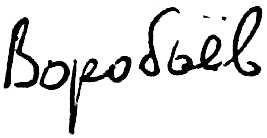
\includegraphics[height=1.5cm]{my_signature} 
\end{flushright}

\vspace{0pt plus3fill} %число перед fill = кратность относительно некоторого расстояния fill, кусками которого заполнены пустые места
\begin{center}
\textbf{\large Воробьев Виталий Сергеевич}
\end{center}

\vspace{0pt plus3fill} %число перед fill = кратность относительно некоторого расстояния fill, кусками которого заполнены пустые места
\begin{center}
\textbf {\Large \MakeUppercase{Модельно-независимое получение CP-нарушающих параметров с использованием когерентных состояний нейтральных D-мезонов}}

\vspace{0pt plus3fill} %число перед fill = кратность относительно некоторого расстояния fill, кусками которого заполнены пустые места
{\large Специальность 01.04.16\ "---\par <<физика атомного ядра и элементарных частиц>>}

\vspace{0pt plus1.5fill} %число перед fill = кратность относительно некоторого расстояния fill, кусками которого заполнены пустые места
\Large{Автореферат}\par
\large{диссертации на соискание учёной степени\par кандидата физико-математических наук}
\end{center}

\vspace{0pt plus4fill} %число перед fill = кратность относительно некоторого расстояния fill, кусками которого заполнены пустые места
\begin{center}
{\large{Новосибирск\ "--- 2016}}
\end{center}

\newpage
% оборотная сторона обложки
%\thispagestyle{empty}
\noindent Работа выполнена в Федеральном государственном бюджетном учреждении науки Институт ядерной физики им. Г.И.~Будкера Сибирского отделения Российской академии наук

\par\vspace{2mm}
    \noindent%
    \begin{tabular}{@{}lp{11cm}}
       Научный руководитель:\\
      \begin{tabular}[t]{@{}l@{}}
        \textbf{Бондарь}\\
        \textbf{Александр Евгеньевич}
      \end{tabular}
      & {доктор физико-математических наук, член-корреспондент РАН, профессор, \par
      ФГБУН Институт ядерной физики им. Г.И.~Будкера СО РАН, г.~Новосибирск, зам. директора
        %\par
        \vspace{3mm} 
        }\\
        { Официальные оппоненты:} & \\
        \begin{tabular}[t]{@{}l@{}}
         \textbf{Николаенко}\\
         \textbf{Владимир Иванович}
        \end{tabular} & 
         кандидат физико-математических наук,\par
         Федеральное государственное бюджетное учреждение «Государственный научный центр Российской Федерации --- Институт физики высоких энергий», г.~Протвино, %\par
         старший научный сотрудник%\par 
         \vspace{2mm}
         \\
        \begin{tabular}[t]{@{}l@{}}
         \textbf{Ростовцев}\\
         \textbf{Андрей Африканович}
        \end{tabular} & 
         доктор физико-математических наук,\par
         Федеральное государственное бюджетное учреждение науки Институт проблем передачи информации им. А.А.~Харкевича Российской академии наук, г.~Москва, %\par
         ведущий научный сотрудник
         \vspace{1mm}
         \\
         Ведущая организация: & Федеральное государственное бюджетное учреждение науки Физический институт им. П.Н.~Лебедева Российской академии наук, г.~Москва
    \end{tabular}  

\par\vspace{2mm}

\noindent Защита состоится~<<26>>~декабря~2016~г.~в~15:45~часов~на~заседании диссертационного совета Д 003.016.02~на базе ФГБУН Института ядерной физики им. Г.И.~Будкера СО РАН~по адресу: 630090, г.~Новосибирск~90, проспект Академика Лаврентьева,~11.

\vspace{2mm}
\noindent С диссертацией можно ознакомиться в библиотеке ФГБУН Института ядерной физики им. Г.И.~Будкера СО РАН, г.~Новосибирск.

\vspace{1mm}
\noindent{Автореферат разослан <<\underline{\ \ \ \ }>> \underline{\ \ \ \ \ \ \ \ \ \ \ \ \ } 2016~г.}

\vspace{2mm}
%\begin{table} [h] % считается не очень правильным использовать окружение table, не задавая caption
%\par\bigskip
    \noindent%
    \begin{tabular}{p{8cm}cr}
        \begin{tabular}{p{8cm}}
            Ученый секретарь  \\
            диссертационного совета % \\
            д-р~физ.-мат. наук
        \end{tabular} 
    &
        \begin{tabular}{c}
%            
\includegraphics[height=1cm]{secretary-signature} 
        \end{tabular} 
    &
        \begin{tabular}{r}
            \\
            \\
            В.С.~Фадин
        \end{tabular} 
    \end{tabular}
%\end{table}
\newpage


\subsection*{Общая характеристика работы}
\textbf{Актуальность темы.} Эксперименты $\belle$ и $\babar$, начавшие в $1999$ году набирать данные на $B$-фабриках \kekb и \pepii, соответственно, существенно продвинули понимание физики тяжелых кварков.  Ключевым результатом работы этих экспериментов стало наблюдение и детальное изучение нарушения \cpconj-симметрии в распадах $B$-мезонов.  Все обнаруженные \cpconj-нарушающие явления находятся в согласии с механизмом \cpconj-нарушения Кобаяши-Маскавы (\km) для слабых заряженных токов.

В некоторых случаях использование многочастичных распадов является необходимым условием для измерения величины параметра (а не установления факта отличия его величины от нуля).  Особенностью таких измерений является необходимость обладать информацией о не наблюдаемой непосредственно фазе амплитуды многочастичного распада.  Амплитуда распада не может быть получена из первых принципов из-за непертурбативных эффектов квантовой хромодинамики.  Эта проблема может быть решена с помощью построения феноменологической модели амплитуды распада и вычисления фазы с помощью этой модели.  
Такой подход, однако, неизбежно приводит к неустранимой и плохо контролируемой модельной неопределенности, которая может стать определяющей при выполнении прецизионных измерений в экспериментах~\lhcb и~\belleii.

Альтернативный подход, в котором среднее значение разности фаз амплитуд распадов \dn- и \dnbar-мезонов для определенной области фазового пространства извлекаются из эксперимента, не требует построения модели.  Этот подход может применяться в экспериментах \lhcb, \belleii, а также на Чарм-Тау-фабрике.

\textbf{Целью}\ данной работы является разработка и доказательство практической реализуемости модельно-независимого подхода к измерению параметров смешивания мезонов и параметров нарушения \cpconj-симметрии с использованием многочастичных распадов $D$- и $B$-мезонов.

Для~достижения поставленной цели необходимо было решить следующие \textbf{задачи}:
\begin{enumerate}
  \item Исследовать влияние осцилляций и прямого нарушения \cpconj-симметрии в распадах $D$-мезонов на измеряемую величину \cpconj-нарушающего параметра \gphi модельно-независимо измеряемую в распадах \bdk, \dkpp.
  \item Разработать модельно-независимый метод получения параметров осцилляций и параметров нарушения \cpconj-симметрии в осцилляциях $D$-мезонов.
  \item Разработать модельно-независимый метод получения параметра \cpconj-нарушения \pphi в распадах \bdh, \dbkpp, $h^0\in\{\pin,\eta^{(\prime)},\omega\}$.
  \item Выполнить модельно-независимое измерение параметра \pphi в вышеупомянутом распаде, используя разработанный метод.
\end{enumerate}

\textbf{Основные положения, выносимые на~защиту:}
\begin{enumerate}
  \item Изучено влияние осцилляций нейтральных $D$-мезонов на наблюдаемую величину параметра \gphi в модельно-независимом измерении в распадах \bdk, \dkpp и предложена процедура, при которой осцилляции $D$-мезонов смещают наблюдаемую величину не более, чем на~$0.2\grad$.
  \item Показано, что в предположении сохранения \cpconj-симметрии в распадах \dnkpp и при существующих экспериментальных ограничениях на величину этого нарушения, смещение наблюдаемой величины \gphi при модельно-независимом измерении в распадах \bdk, \dkpp, не превосходит $3\grad$.
  \item Показано, что модельно-независимое получение параметра \gphi в распадах \bdk, \dkpp возможно без предположения сохранения \cpconj-симметрии в распадах \dnkpp; при этом не наблюдается существенного снижения статистической чувствительности.
  \item Предложен метод модельно-независимого измерения параметров смешивания и \cpconj-нарушения в смешивании нейтральных $D$-мезонов в процессе $\ep\to \ddbar{}^{*}$ без измерения времени распада~$D$.
  \item Предложен метод модельно-независимого получения параметров смешивания и \cpconj-нарушения в смешивании нейтральных $D$-мезонов в процессе \dstpdpip, \dnkpp с измерением времени распада~$D$.
  \item Предложен метод модельно-независимого измерения \cpconj-нарушающей фазы \pphi в распадах \bdsth, \dbkpp; данный метод позволяет разрешить неопределенность, присущую измерению $2\pphi$ в переходах~\btoccs.
  \item Впервые выполнено модельно-независимое измерение фазы \pphi в распадах \bdsth, \dbkpp и получен результат $\pphi = 11.7\grad\pm7.8\grad\pm2.1\grad$, позволяющий разрешить неопределенность значения $2\pphi$ на уровне достоверности, превышающем $5$ стандартных отклонений.
  \item Подготовлен алгоритм для автоматического измерения характеристик модуля усилителя-формирователя калориметра \belleii, который был использован для проверки характеристик всех изготовленных модулей.
\end{enumerate}

\textbf{Научная новизна:}\ впервые выполнено модельно-независимое измерение параметра~\pphi в распадах~\bdsth, \dbkpp; впервые предложены свободные от модельной неопределенности методы измерения параметров смешивания $D$-мезонов и~\cpconj-нарушающего параметра~\pphi с использованием многочастичных распадов нейтральных $D$-мезонов.

\textbf{Практическая значимость}: предложенный метод измерения параметра~\pphi, а также результаты исследования процедуры модельно-независимого измерения параметра~\gphi используются и будут использоваться при выполнении прецизионных измерений в экспериментах~\babar, \belle, \belleii и~\lhcb.  Предложенный метод измерения параметров осцилляций $D$-мезонов может быть использован при выполнении измерений в эксперименте~\besiii и в будущих экспериментах на Чарм-Тау-фабрике.

\textbf{Достоверность}\ полученных результатов обеспечивается публикацией основных результатов в рецензируемых журналах с высокой цитируемостью. Результаты измерения параметра~\pphi находятся в согласии с предыдущим измерением в эксперименте~\belle, а также с результатом измерения, выполненного группой~\babar.

\textbf{Апробация работы.}\ Основные результаты работы докладывались~на научных семинарах в ИЯФ СО РАН и KEK (Цукуба, Япония).  Результаты измерения параметра \pphi были доложены на конференциях XIII Heavy Quarks and Leptons conference (HQL 2016) и 38th International Conference On High Energy Physics (ICHEP 2016).

\textbf{Личный вклад.}\ Изложенные в работе результаты получены автором лично либо при его определяющем вкладе.

\textbf{Публикации.} Основные результаты по теме диссертации изложены в 5 печатных изданиях, 5 из которых изданы в журналах, рекомендованных~ВАК.

{\textbf{Объем и структура работы.}} Диссертация состоит из~введения, четырех глав, заключения и пяти~приложений. Объем диссертации составляет $172$~страницы текста с~$59$~рисунками и~$19$~таблицами. Список литературы содержит $138$~наименований.

%%%%%%%%%%%%%%%%%%%%%%%%%%%%%%%%%%%%%%%%%%%%%%%%%%%%%%%%%%%%%%%%
%%%%%%%%%%%%%%%%%%%%%%%%%%%%%%%%%%%%%%%%%%%%%%%%%%%%%%%%%%%%%%%%
%%%%%%%%%%%%%%%%%%%%%%%%%%%%%%%%%%%%%%%%%%%%%%%%%%%%%%%%%%%%%%%%

\subsection*{Содержание работы}
Во {\textbf{введении}} обосновывается актуальность исследований, проводимых в рамках данной диссертационной работы, формулируется цель, ставятся задачи работы, сформулированы научная новизна и практическая значимость представляемой работы.

{\textbf{Первая глава}} посвящена рассмотрению основных феноменологических подходов к изучению нарушения \cpconj-симметрии в ускорительных экспериментах и описанию экспериментального статуса изучения нарушения \cpconj-симметрии.

В рамках Стандартной Модели (СМ) нарушение \cpconj-симметрии (\cpconj-нарушение) описывается механизмом Кобаяши-Маскавы (\km), согласно которому лагранжиан слабых заряженных токов описывает взаимодействие кварковых полей $q_u$ и $q_b^{\prime}$, где $q_u=\{u, c, t\}$ --- вектор полей верхних кварков, а $q_b^{\prime} = \{d^{\prime}, s^{\prime}, b^{\prime}\}$ --- вектор линейных комбинаций полей нижних кварков:
\begin{equation}\label{eq:ckm}
 \left(
 \begin{array}{c}
   d^{\prime} \\
   s^{\prime} \\
   b^{\prime} \\
  \end{array}
  \right)
  = \vckm
  \left(
  \begin{array}{c}
   d \\ s \\ b \\
  \end{array}
  \right)
  =
  \left(
  \begin{array}{ccc}
   V_{ud} & V_{us} & V_{ub} \\
   V_{cd} & V_{cs} & V_{cb} \\
   V_{td} & V_{ts} & V_{tb} \\
  \end{array}
  \right)\left(
  \begin{array}{c}
   d \\ s \\ b \\
  \end{array}
  \right),
\end{equation}
где $\vckm$ --- унитарная матрица смешивания кварков, называемая матрицей Кабиббо-Кобаяши-Маскавы~(\ckm).  Матрица смешивания антикварков получается комплексным сопряжением матрицы~\vckm.  Взаимодействие кварков отличается от взаимодействия антикварков, если $\vckm^*\neq \vckm$.  Матрица~\vckm задается тремя углами Эйлера и фазой~$\delta$, которая является единственным параметром СМ, отвечающим за \cpconj-нарушение.

Экспериментальная проверка механизма~\km сводится к измерению величин элементов и проверке условия унитарности матрицы~\ckm.  Наиболее подходящим для экспериментальной проверки является соотношение
\begin{equation}\label{eq:ut}
 \frac{V_{ud}V_{ub}^*}{V_{cd}V_{cb}^*}+\frac{V_{td}V_{tb}^*}{V_{cd}V_{cb}^*} + 1 = 0,
\end{equation}
которое можно представить в виде треугольника на комплексной плоскости (рисунок~\ref{fig:UT}), называемого Треугольником Унитарности (\ut). Величины углов~\ut выражаются через элементы матрицы~\ckm следующим образом:
\begin{equation}\label{eq:ut_angles}
 \aphi = \arg\lbr-\frac{V_{td}V^*_{tb}}{V_{ud}V^*_{ub}}\rbr,\quad
 \pphi = \arg\lbr-\frac{V_{cd}V^*_{cb}}{V_{td}V^*_{tb}}\rbr,\quad
 \gphi = \arg\lbr-\frac{V_{ud}V^*_{ub}}{V_{cd}V^*_{cb}}\rbr.
\end{equation}

\begin{figure}[h]
 \centering
  \includegraphics[width=0.5\textwidth]{UT}
   \caption{Геометрическое представление соотношения~\eqref{eq:ut}.}
  \label{fig:UT}
\end{figure}

Величины всех углов и сторон \ut можно определить из наблюдений. Получившаяся переопределенная система ограничений позволяет выполнить прецизионную проверку соотношений треугольника для \ut.  Анализ показывает, что при текущей точности измерения параметров \ut, составляющей в среднем $5\%$-$10\%$, значимых нарушений СМ не выявлено.  Таким образом, необходимо дальнейшее повышение точности измерений.

%%%%%%%%%%%%%%%%%%%%%%%%%%%%%%%%%%%%%%%%%%%%%%%%%%%%%%%%%%%%%%%%%%%
%%%%%%%%%%%%%%%%%%%%%%%%%%%%%%%%%%%%%%%%%%%%%%%%%%%%%%%%%%%%%%%%%%%
%%%%%%%%%%%%%%%%%%%%%%%%%%%%%%%%%%%%%%%%%%%%%%%%%%%%%%%%%%%%%%%%%%%

{\textbf{Вторая глава}} посвящена описанию модельно-независимого подхода к анализу многочастичных распадов.  В этой главе предложены программы исследований для симметричной Чарм-Тау-фабрики и асимметричной $B$-фабрики, а также для эксперимента \lhcb, основанные на этом подходе.  

Гири с соавторами предложили идею модельно-независимого получения угла~\gphi~\ut в распадах \bdk, \dkpp.  Предложение состоит в использовании среднего значения разности фаз $\deld$ амплитуд распадов $\ad\equiv\mca\lbr\dnkpp\rbr$ и $\adbar\equiv\mca\lbr\dbkpp\rbr$ для нескольких областей фазового пространства:
\begin{equation}\label{eq:csi}
  \zi \equiv \ci + i\si = 
            \frac{\int\ddlzarea
            \left|\ad\right|\left|\adbar\right|
            e^{i\deld}\,\ddlz}
            {\int\ddlzarea\left|\ad\right|^2 \ddlz 
             \int\ddlzarea\left|\adbar\right|^2 \ddlz}
            ,
\end{equation}
где индекс $i$ обозначает номер области фазового пространства, $\mcd$ обозначает полное фазовое пространство, $\mcd_i$ обозначает область фазового пространства, соответствующую номеру~$i$ и $m^2_{\pm}\equiv m^2\lbr\ks\pi^{\pm}\rbr$ обозначают квадраты масс пар частиц конечного состояния (переменные Далица).  Параметры \ci и \si близки по смыслу к среднему в $i$-й области значению $\cos\deld$ и $\sin\deld$, соответственно.  Кроме того, вводят параметры \ki и \kbi,  обозначающие вероятность попадания события в $i$-ю область при распаде \dn- и \dnbar-мезона, соответственно.  Для произвольного разбиения значения параметров \ki, \kbi, \ci и \si могут быть получены в когерентных распадах $\dn\dnbar$ на симметричном коллайдере, работающем вблизи резонанса \ppsi.

Предполагая отсутствие \cpconj-нарушения в распадах $D$-мезонов, т.е. используя соотношение $\ad\dvar\equiv\adbar\dvarinv$, можно оптимизировать способ разбиения диаграммы Далица распада \dnkpp: выбрать $2\mcn$ области симметрично относительно перестановки $\mpsq\leftrightarrow\mmsq$.  Номера областей $i$ при этом принимают значения от $-\mcn$ до $\mcn$, исключая $0$, такие, что инверсия знаков номеров областей $i\to -i$ соответствует перестановке $\mpsq\leftrightarrow\mmsq$. При таких договоренностях выполняются соотношения
\begin{equation}\label{eq:cp-conserv-relations}
 \zi \equiv Z^*_{-i}\quad (C_i\equiv C_{-i},\quad S_i\equiv -S_{-i}),\quad \kbi \equiv \kmi.
\end{equation}
Форму областей разумно выбрать так, чтобы получить максимальную статистическую чувствительность к измеряемым параметрам.  Хорошее приближение к оптимальному способу разбиения дает критерий
\begin{equation}\label{eq:uniph}
 \frac{2\pi\left(i-\frac{1}{2}\right)}{\mcn} < \deld\dvar < \frac{2\pi\left(i+\frac{1}{2}\right)}{\mcn}\quad
 \left(\textrm{для}\ \mpsq>\mmsq\ \textrm{и}\ i>0\right).
\end{equation}
Полученное таким способом разбиение называют \emph{равномерным по фазе}.  Критерий~\eqref{eq:uniph} может быть использован только на основе модельных соображений, поскольку функция $\deld\dvar$ неизвестна.  Такое использование модели, однако, не приводит к систематической ошибке измерения.

\begin{figure}[htb]
\begin{minipage}[b]{0.5\textwidth}
 \centering
  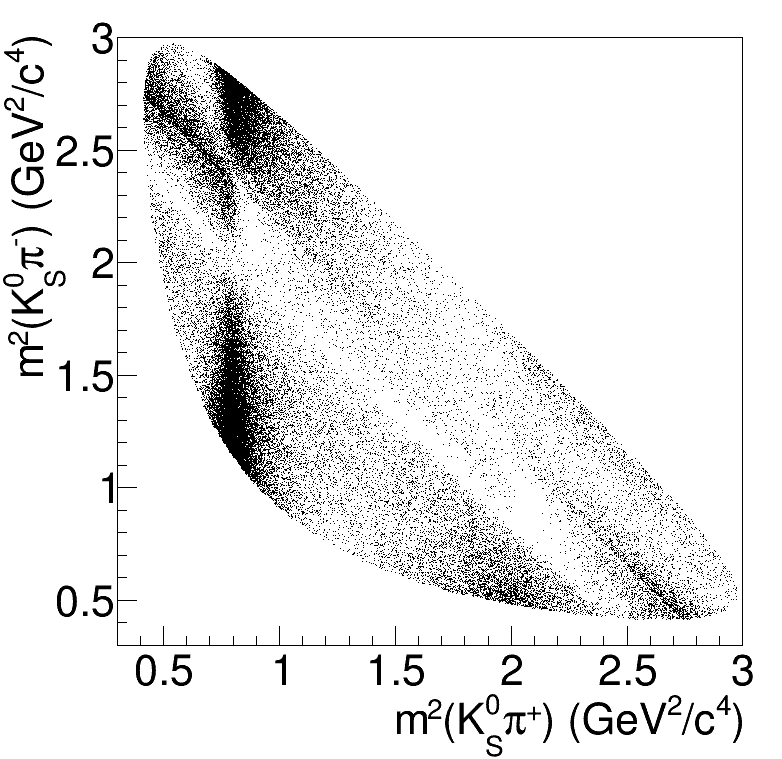
\includegraphics[width=0.85\textwidth]{dp_mc.png}
 \subcaption{}
 \label{fig:dalitz}
\end{minipage}
\begin{minipage}[b]{0.5\textwidth}
 \centering
  \includegraphics[width=0.9\textwidth]{belle_eqdel_bins}
 \subcaption{}
 \label{fig:bd_belle_eqph}
\end{minipage}
 \caption{а) Диаграмма Далица для распада \dbkpp и б)~равномерное по фазе разбиение этой диаграммы, выполненное с помощью модели, полученной с данными детектора \belle.}
 \label{fig:dalitz_plot}
\end{figure}

На рисунке~\ref{fig:dalitz_plot} показано распределение по переменным Далица (диаграмма Далица) для распада \dbkpp и равномерное по фазе разбиение, выполненное на основе полученной в эксперименте \belle модели.  

\paragraph{\boldmath Получение параметров смешивания в когерентных распадах $D$-мезонов.  }  Осцилляции $D$-мезонов описывают \emph{параметры смешивания}
\begin{equation}
 x_D \equiv \frac{\Delta m_D}{\Gamma_D},\quad y_D \equiv \frac{\Delta\Gamma_D}{2\Gamma_D},
\end{equation}
где $\Delta m_D$ ($\Delta\Gamma_D$) обозначает разность масс (ширин) массовых состояний нейтральных $D$-мезонов и $\Gamma_D$ обозначает полусумму ширин этих состояний.  Параметры смешивания малы $x_D\sim y_D\sim 10^{-2}$, поэтому мы всюду используем разложение в ряд по этим параметрам.

Параметры смешивания могут быть получены модельно-независимым образом в когерентных распадах пар $\dn\dnbar$, находящихся в симметричном по перестановке состоянии с $\cconj=+1$.\footnote{Для наглядности мы предполагаем сохранение \cpconj-симметрии в смешивании $D$-мезонов, хотя обсуждаемые ниже методы позволяют получить параметры \cpconj-нарушения в смешивании вместе с параметрами смешивания $D$-мезонов, если рассмотреть более общий формализм.}  Такие пары можно получить в распадах $\ep\to \dn\dbar{}^{*0}$, $\dbar{}^{*0}\to\dnbar\gamma$.  Пусть один из $D$-мезонов такой пары переходит в состояние~\kspp.  Вероятность попадания в область диаграммы Далица с индексом~$i$ при этом зависит от типа конечного состояния второго $D$-мезона.  При переходе второго $D$-мезона в \cpconj-собственное состояние с \cpconj-четностью~$\eta_D$ эта вероятность задается выражением
\begin{equation}\label{eq:m_cp_sym}
  \left<M^{\cconj+}_{i,\eta_D}\right> 
  \propto \lbr\ki+\kmi\rbr\lbr1 + 2\eta_D y_D\rbr + 2\ci\sqrt{\ki\kmi}\lbr\eta_D + 2y_D\rbr
  + \oxdydsq.
\end{equation}
Соответствующая вероятность при переходе второго $D$-мезона в состояние с определенным ароматом:
\begin{equation}\label{eq:m_flv_sym}
 \left<M^{\cconj+}_{i}\right> 
 \propto \ki + 2\sqrt{\ki\kmi}\lbr y_D\ci+x_D\si\rbr + \oxdydsq.
\end{equation}
Дополнительно можно рассмотреть некогерентный переход \dnbar-мезона, рожденного в процессе $\ep\to D^+D^{-*}$, $D^{-*}\to\dnbar\pi^+$, в состояние \kspp.  Вероятность попадания в область номер $i$ в этом случае:
\begin{equation}\label{eq:kprime}
 \ki^{\prime} \propto \ki + \sqrt{\ki\kmi}\lbr y_D\ci + x_D\si\rbr + \oxdydsq.
\end{equation}
При известных значениях параметров \ki, \ci и \si соотношения~\eqref{eq:m_cp_sym}, \eqref{eq:m_flv_sym} и~\eqref{eq:kprime} позволяют получить параметры смешивания $x_D$ и $y_D$.  

В процессе $\ep\to \dn\dbar{}^{*0}$, $\dbar{}^{*0}\to\dnbar\pin$ образуется когерентная пара~$\dn\dnbar$-мезонов в антисимметричном состоянии с $\cconj=-1$, которое позволяет получить не искаженные смешиванием значения параметров~\ki, \ci и~\si.  Таким образом, рассматривая совместно распады~$\dbar{}^{*0}\to\dnbar\pin$ и~$\dbar{}^{*0}\to\dnbar\gamma$, можно выполнить измерения, достаточные для получения параметров смешивания $D$-мезонов.  Оптимальной энергией коллайдера для предложенного измерения является~$4.01\gev$, которая находится под порогом рождения~$D^*\dbar{}^*$-пар.  Численные эксперименты показывают, что параметры смешивания могут быть получены с точностью около $10^{-3}$ с данными, соответствующими году работы Чарм-Тау-фабрики со светимостью~$10^{35}\lumi$.

\paragraph{\boldmath Получение параметров смешивания в некогерентных распадах $D$-мезонов с измерением времени распада. } Плотность вероятности перехода \dn-мезона, рожденного в процессе \dstpdpip, в состояние \kspp при условии попадания в $i$-ю область диаграммы Далица:
\begin{equation}\label{eq:kprime-time}
 \ki^{\prime}\lbr t\rbr \propto \dexp\left[ \ki+\sqrt{\ki\kmi}\lbr y_D\ci+x_D\si\rbr\Gamma t+ \oxdydtsq \right].
\end{equation}
Соотношение~\eqref{eq:kprime-time} впервые опубликовано в работе автора диссертации и позволяет получить параметры \ki и параметры смешивания $D$-мезонов во времязависимых измерениях на $B$-фабрике или в эксперименте~\lhcb.  Как уже обсуждалось, значения параметров~\ci и~\si могут быть получены независимо.  Первое получение параметров смешивания описанным методом было выполнено недавно группой~\lhcb. 

\paragraph{\boldmath Влияние смешивания $D$-мезонов и прямого \cpconj-нарушения в распаде \dnkpp на получение угла \gphi. } В перспективе прецизионного модельно-независимого получения угла~\gphi в экспериментах~\belleii и~\lhcb важным вопросом является влияние осцилляций $D$-мезонов на величину~\gphi, полученную модельно-независимом способом в распадах \bdk, \dkpp.  Мы рассмотрели две процедуры: согласно первой процедуре для определения~\gphi используются значения параметров~\ki, \ci и~\si, полученные в когерентных распадах $\dn\dnbar$-пар; вторая процедура отличается от первой тем, что значения параметров~\ki получены в некогерентных распадах, и поэтому искаженны смешиванием (смотрите уравнение~\eqref{eq:kprime}).  

Смещение \gphi для обоих процедур оценено с помощью численных экспериментов.  Первая процедура (\ki получены в когерентных распадах) приводит к смещению, не превышающему
\begin{equation}
 \delta\gphi^{(\mathrm{max})} = 3\grad\times \frac{\sqrt{x_D^2+y_D^2}}{0.1\rb}\approx 3\grad,\quad \rb = \left|\frac{\mca\lbr B^+\to\dn K^+\rbr}{\mca\lbr B^+\to\dnbar K^+\rbr}\right|.
\end{equation}
При использовании второй процедуры вклад смешивания в вероятность попадания события в область фазового пространства с индексом $i$ дополнительно подавлен фактором порядка \rb и максимальное смещение составляет
\begin{equation}
 \delta\gphi^{(\mathrm{max})} \approx 3\grad\times\rb\times \frac{\sqrt{x_D^2+y_D^2}}{0.1\rb}\approx 0.2\grad.
\end{equation}
Полученные результаты позволяют заключить, что получение параметров~\ki в некогерентных распадах позволяет не учитывать смешивание $D$-мезонов даже при прецизионном модельно-независимом получении~\gphi в эксперименте~\belleii (точность которого может быть близка к $1\grad$).  

С помощью численных экспериментов изучено влияние прямого \cpconj-нарушения в распадах \dnkpp на извлекаемую модельно-независимым способом величину угла~\gphi в распадах~\bdk, \dkpp.  Показано, что смещение~\gphi не превосходит $3\grad$.  Эта величина определяется точностью экспериментального ограничения величины \cpconj-нарушения в распадах \dnkpp, полученного в эксперименте~CDF.  Ожидается, что измерения в экспериментах \lhcb и \belleii позволят значительно уменьшить эту величину, поскольку в СМ не ожидается значимых \cpconj-нарушающих эффектов в распадах $D$-мезонов.  

Кроме того, показано, что угол \gphi может быть извлечен в распадах \bdk, \dkpp модельно-независимо и без предположения сохранения \cpconj-симметрии в распадах \dnkpp. При этом статистическая чувствительность метода уменьшается незначительно.

\paragraph{\boldmath Модельно-независимое получение угла \pphi. }  Бондарь, Гершон и Кроковный предложили получать угол \pphi в распадах \bdsth, \dbkpp, $h\in\{\pin\eta^{(\prime)},\omega\}$.  Этот метод позволяет разрешить дискретную неопределенность $2\pphi\to\pi-2\pphi$, присущую классическому получению величины \sindbeta в кварковых переходах \btoccs.  Модельно-независимая модификация этого метода, предложенная автором диссертации, приводит к следующему выражению для плотности вероятности распада в~$i$-й области:
\begin{equation}\label{eq:master-formula}
 \begin{split}
  \mcp_i\lbr \dt\rbr &\propto \bexp\left[ 1 + q_B\frac{\ki-\kmi}{\ki+\kmi}\cos\dmdt\right.\\
  &\left.+2q_B\eta_{h^0}(-1)^l\frac{\sqrt{\ki\kmi}}{\ki+\kmi}\sin\dmdt\left(\si\cosdbeta+\ci\sindbeta\right)\right],
 \end{split}
 \end{equation} 
где $\dt$ обозначает разность собственных времен распада сигнального и помечающего $B$-мезонов, $q_B = 1$ ($q_B = -1$) соответствует аромату~\bn~(\bnbar) сигнального $B$-мезона при~$\dt=0$, $\eta_{h^0}$ обозначает \cpconj-четность $h^0$-мезона и $l$ обозначает орбитальный момент $Dh^0$-системы.\footnote{Для распадов \bdstarh, \dbstdbpi, \dbkpp в функции \mcs возникает дополнительный множитель $-1$.}  

{\textbf{Третья глава}} посвящена описанию асимметричного электрон-позитронного ускорителя \kekb и детектора \belle.  В этой главе также обсуждается участие автора в модернизации калориметра детектора \belle для подготовки работы калориметра в эксперименте \belleii.  

В {\textbf{четвертой главе}} обсуждается выполненное впервые модельно-независимое измерение угла~\pphi в распадах \bdsth, \dbkpp, $h^0\in\{\pin, \eta, \etap, \omega\}$ (смотрите уравнение~\eqref{eq:master-formula}).  Для измерения использован полный интеграл светимости $711\ifb$, набранный детектором~\belle вблизи резонанса~\ups, соответствующий $771$ миллионам $\ups\to\bbbar$-событий.  Равномерное по фазе разбиение фазового пространства распада \dnkpp выполнено с помощью модели, полученной ранее в эксперименте~\belle.  Значения параметров \ci и \si для этого разбиения были измерены в эксперименте CLEO.  Значения параметров \ki получены с помощью распадов \bpdpi, \dbkpp.

Процедура анализа событий состоит из нескольких основных этапов.  На первом этапе происходит отбор кандидатов \bdsth с помощью различных кинематических параметров, изучение компонент фона и применение классифицирующих алгоритмов для подавления фона.  На втором этапе для каждого реконструируемого распада определяется доля сигнальных событий посредством анализа двумерного распределения параметров~\de и~\mbc:
\begin{equation}
 \de=E_B^{\cms}-E_{\mathrm{beam}}^{\cms},\quad
 \mbc = \sqrt{\left(E^{\cms}_{\mathrm{beam}}\right)^2-\left(p^{\cms}_{B}\right)^2},
\end{equation}
где $E_B^{\cms}$, $p^{\cms}_{B}$ и $E_{\mathrm{beam}}^{\cms}$ обозначают соответственно энергию $B$-кандидата, импульс $B$-кандидата и энергию пучка в системе центра масс.  Форма сигнального и фонового распределений \de-\mbc изучаются с помощью моделирования.  Заключительный этап анализа состоит анализе распределений по~\dt.  Фоновые \dt-распределения предварительно изучаются с помощью моделирования, а затем уточняются с помощью экспериментальных событий.  Корректность описания фоновых \dt-распределений и функции разрешения по \dt для сигнальных событий контролируется посредством измерения времени жизни \bn-мезона в распадах \bdsth, \dbkpp.  Получение \cpconj-нарушающих параметров осуществляется методом максимального правдоподобия с функцией правдоподобия вида
\begin{equation}\label{eq:lh}
 \mcl(\xi) = \prod\limits_{j=1}^{N}\left[\fsigj\psig\lbr\dtj,\xi\rbr+\lbr 1-\fsigj\rbr\pbkg\lbr\dtj\rbr\right],
\end{equation}
где $N$ обозначает количество отобранных событий, $\psig$ ($\pbkg$) обозначает плотность вероятности для сигнальных (фоновых) событий, $\fsigj$ обозначает вероятность того, что событие $j$ является сигнальным и $\xi\in\{\sindbeta, \cosdbeta, \pphi\}$.  Границы (асимметричных) доверительных интервалов $[\xi_{\mathrm{nl}},\xi_{\mathrm{nr}}]$, соответствующие $n$ стандартным отклонениям, определяются условием
\begin{equation}
 n^{2} = -2\log\lambda(\xi_{\mathrm{nl}}) = -2\log\lambda(\xi_{\mathrm{nr}}),
\end{equation}
где $\xi_{\mathrm{nl}}$ ($\xi_{\mathrm{nr}}$) обозначает левую (правую) границу интервала и $-2\log\lambda(\xi)$ обозначает логарифм отношения вероятностей 
\begin{equation}\label{eq:confidence_intervals}
 -2\log\lambda(\xi)=-2\log\mcl(\xi,\hat{\hat{\vecp}}) + 2\log\mcl(\hat{\xi},\hat{\vecp}).
\end{equation}
Здесь \vecp обозначает множество параметров за исключением~$\xi$, от которых зависит функция правдоподобия~$\mcl$, $\hat{\xi}$ и $\hat{\vecp}$ обозначают значения параметров, минимизирующее функцию правдоподобия, $\hat{\hat{\vecp}}$ обозначает значения параметров, минимизирующие функцию правдоподобия для текущего значения~$\xi$.  На рисунке~\ref{fig:lambda} показаны логарифмы отношения вероятностей для \cpconj-нарушающих параметров.  Следующие значения соответствуют одному стандартному отклонению:
 \begin{equation}\label{eq:final_results}
 \begin{split}
  \sindbeta &= 0.43     \pm 0.27\stat    \pm 0.08    \syst,\\
  \cosdbeta &= 1.06     \pm 0.33\stat^{+0.21}_{-0.15}\syst,\\
  \pphi     &= 11.7\grad\pm 7.8\grad\stat\pm 2.1\grad\syst.
 \end{split}
 \end{equation}

Величина $\sindbeta=0.691\pm0.017$, полученная в кварковых переходах \btoccs, определяет абсолютное значение \cosdbeta, которому соответствуют два значения угла $\pphi\in[0\grad; 180\grad)$.  Представленное в данной работе измерение исключает отрицательное значение \cosdbeta, соответствующее $\pphi = 68.1\grad$, на уровне $5.1$ стандартных отклонений и находится в согласии с положительным значением \cosdbeta, соответствующим значению $\pphi = 21.9\grad$ на уровне $1.3$ стандартных отклонений.  Таким образом, представленное измерение разрешает неопределенность в значении угла \pphi, присущую измерению параметра \sindbeta в переходах \btoccs.

\begin{figure}[htb]
 \begin{minipage}[b]{0.32\textwidth}
  \centering
  \includegraphics[width=\textwidth]{sin_minos_errors_v4}
  \subcaption{}
 \end{minipage}
 \begin{minipage}[b]{0.32\textwidth}
  \centering
  \includegraphics[width=\textwidth]{cos_minos_errors_v4}
  \subcaption{}
 \end{minipage}
 \begin{minipage}[b]{0.32\textwidth}
  \centering
  \includegraphics[width=\textwidth]{phi1_minos_errors_v4}
  \subcaption{}
 \end{minipage}
  \caption{Логарифмы отношений вероятностей~\eqref{eq:confidence_intervals} для а)~\sindbeta, б)~\cosdbeta и в)~\pphi. Квадраты (круги) показывают значения без учета (с учетом) систематических неопределенностей.  Пунктирные и непрерывные линии показывают аппроксимацию полученных значений.  Вертикальные линии показывают значения, соответствующие $\sindbeta=0.691$.  }
  \label{fig:lambda}
\end{figure}

Доминирующие систематические неопределенности представленного измерения имеют статистическую природу.  Основной вклад вносит неопределенность значений параметров~\ci и~\si, полученных в эксперименте~CLEO.  Эти неопределенности могут быть уменьшены с помощью измерений в эксперименте~\besiii.  Другие существенные неопределенности связаны с описанием временного разрешения и распределений по параметрам~\de и~\mbc.  Эти неопределенности зависят от статистики и будут меньше при выполнении измерения в эксперименте~\belleii.  При выполнении описанного анализа, таким образом, показано отсутствие систематических неопределенностей, потенциально ограничивающих точность прецизионного измерения в эксперименте~\belleii.

В {\textbf{заключении}} приведены основные результаты работы и кратко описаны перспективы развития и практической реализации предложенных в работе методов модельно-независимого получения параметров в экспериментах \belleii, \lhcb и на Чарм-Тау-фабрике.

\large{Публикации автора по теме диссертации}

\begin{enumerate}
 \item A.~Bondar, A.~Poluektov, V.~Vorobiev Charm mixing in a model-independent analysis of correlated $\dn\dnbar$ decays // Phys. Rev. D. --- 2010. --- Aug. --- Vol. 82, issue 3. --- P. 034033. --- DOI: \verb@10.1103/PhysRevD.82.034033@.
 \item Effect of direct CP violation in charm on γ extraction from $\bdk$, $\dkpp$ Dalitz plot analysis / A.~Bondar, A.~Dolgov, A.~Poluektov and V.~Vorobiev // The European Physical Journal C. --- 2013. --- Vol. 73, no. 6. --- Pp. 1--6. --- DOI: \verb@10.1140/epjc/s10052-013-2476-9@.
 \item Measurement of the CKM angle $\varphi_1$ in $\bdsth$, $\dbkpp$ decays with time-dependent binned Dalitz plot analysis / V.~Vorobyev, I.~Adachi, H.~Aihara, [et al.] // Phys. Rev. D. --- 2016. --- Sept. --- Vol. 94, issue 5. --- P. 052004. --- DOI: \verb@10.1103/PhysRevD.94.052004@.
 \item Testbench of shaper-digitizer modules for Belle II calorimeter / V.~Vorobyev, A.~Kuzmin, D.~Matvienko and A.~Vinokurova // Journal of Instrumentation. --- 2014. --- Vol. 9, no. 08. --- P. C08016. --- DOI: \verb@10.1088/1748-0221/9/08/C08016@.
 \item First measurement of φ 3 with a model-independent Dalitz plot analysis of $\bdk$, $\dkpp$ decay / H.~Aihara, K.~Arinstein, D.M.~Asner, [et al.] // Phys. Rev. D. --- 2012. --- June. --- Vol. 85, issue 11. --- P. 112014. --- DOI: \verb@10.1103/PhysRevD.85.112014@.
\end{enumerate}


\end{document}